%% appendix.tex
%%

%% ==============================
%\chapter{Appendix}
%\label{ch:Appendix}
%% ==============================

\appendix

\iflanguage{english}
{\addchap{Appendix}}	% english style
{\addchap{Anhang}}	% german style

\section{Algorithm}
		\label{Appendix-Algorithm}
		
\begin{algorithm}[h] % setup Rounds
\LinesNumbered
\SetNoFillComment
\setcounter{AlgoLine}{0}
 \SetAlgoLined
 \tcc{rounds:= 4 rounds; 4 usergroups}
  \KwIn{rounds, usergroups }
 \KwResult{4 Rounds per each usergroup }

 benchmarkCurrent = 0\;
 
\ForAll{rounds}{
\tcc{100 iterations}
 \For{i=0 to 100}{
 \tcc{100 Boxes}
 \For{j=0 to 100}{
 	width = uniform random in range of 20 and 80\;
 	

 	benefit = uniform random in range of 0 and 80\;
 	
 	create Box with width and benefit
 }\;

benchmark = (\ac{DPA} Solution / \ac{GA} Solution\ - 1) x 100\%;
 
 \If{benchmarkCurrent $\leq$ benchmark}{
 	benchmarkCurrent = benchmark
 	
 	  \tcc{itemsHardProblem:= save current boxes }
 
 	boxesHardProblem = boxes
 	}
 }

 \ForAll{ boxes in boxesHardProblem}{
 \ForAll{usergroups}{
 new Box (box.benefit, box.weight, current round)\;
 
 add colour according to benefit and number of colours\;
} 	
 } }
\caption{Setup of rounds}
\label{Setup of rounds}
\end{algorithm}

\newpage
\section{Interface for each usergroup}
		\label{Appendix-Implementation}
		
\setcounter{figure}{0}
\begin{figure}[htbp] % DistributionFinalResult
\begin{center} 
\begin{subfigure} 
\centering
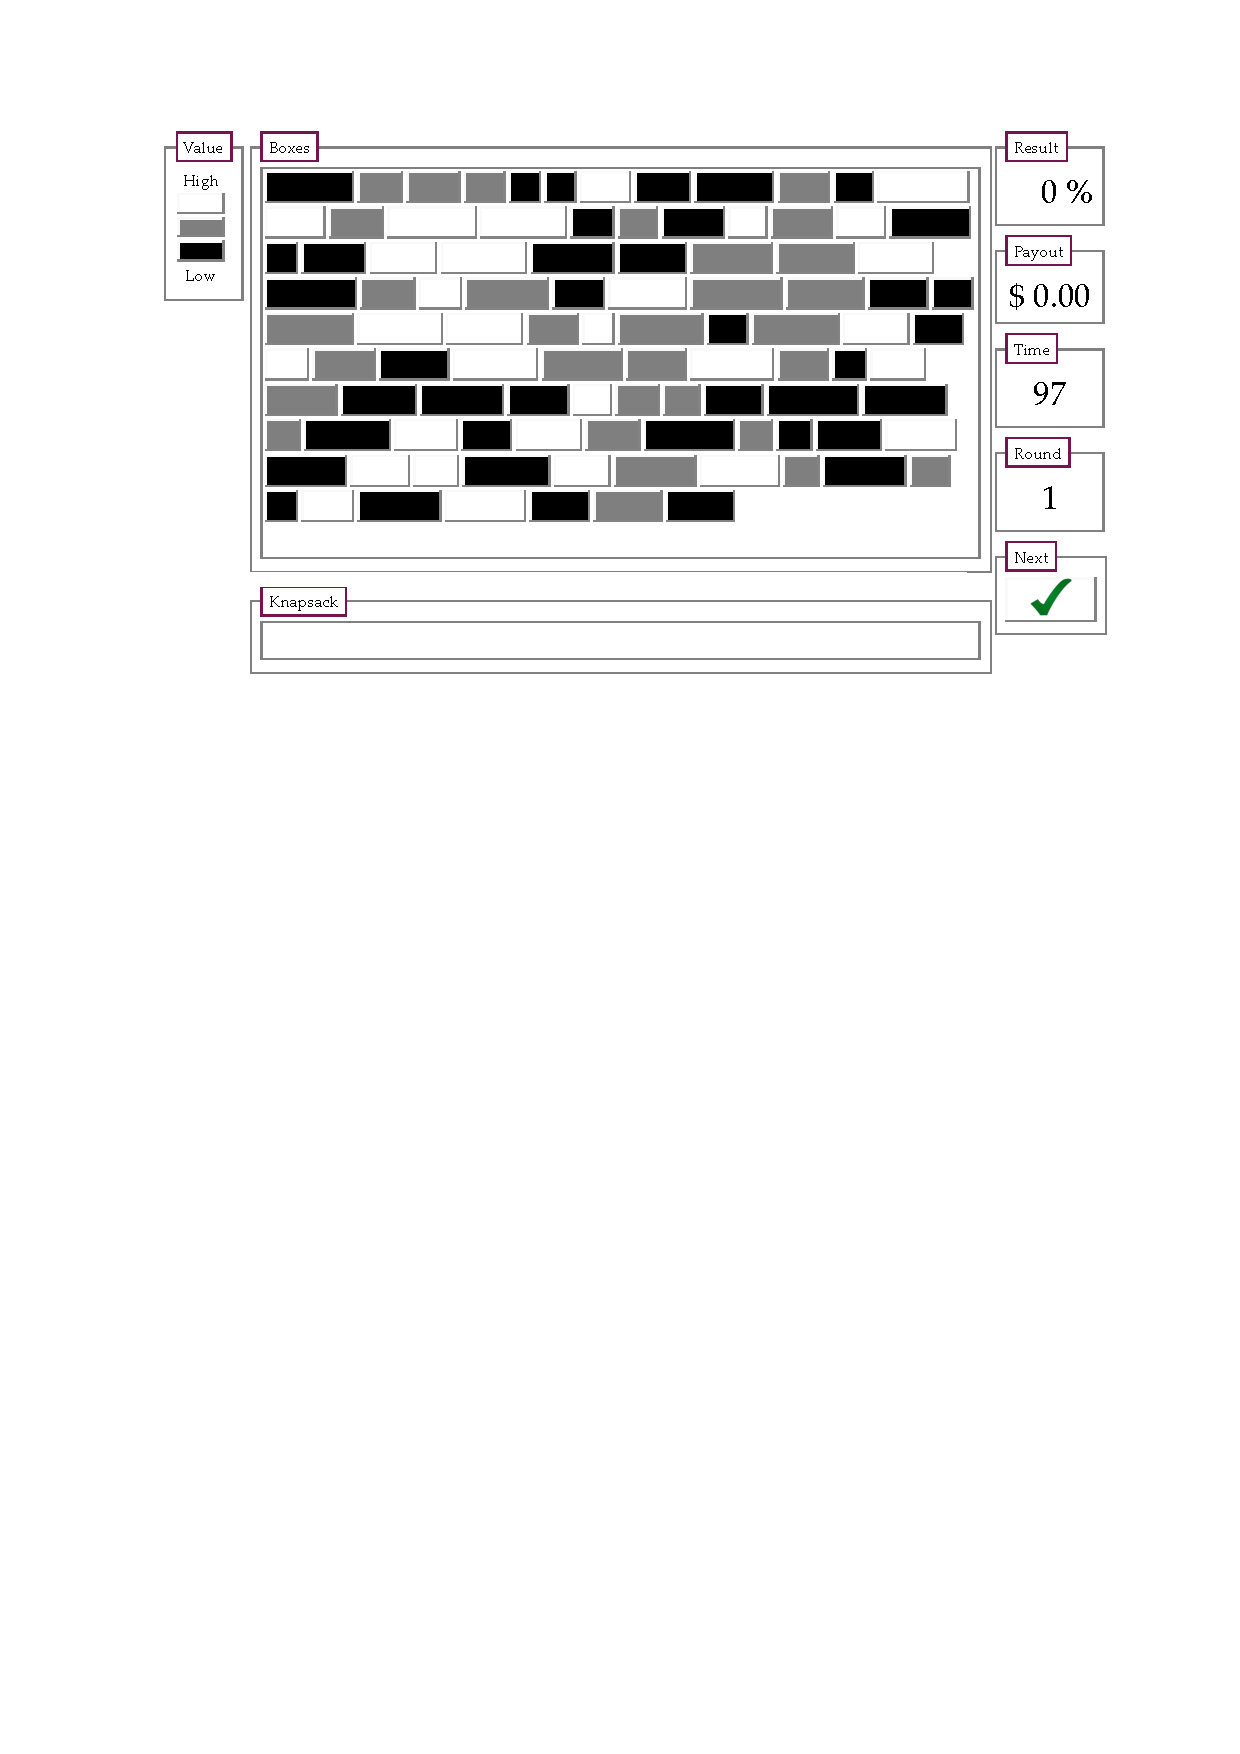
\includegraphics[height = 0.39\textwidth]{Interface1.pdf}
\end{subfigure} 
\begin{subfigure} 
\centering
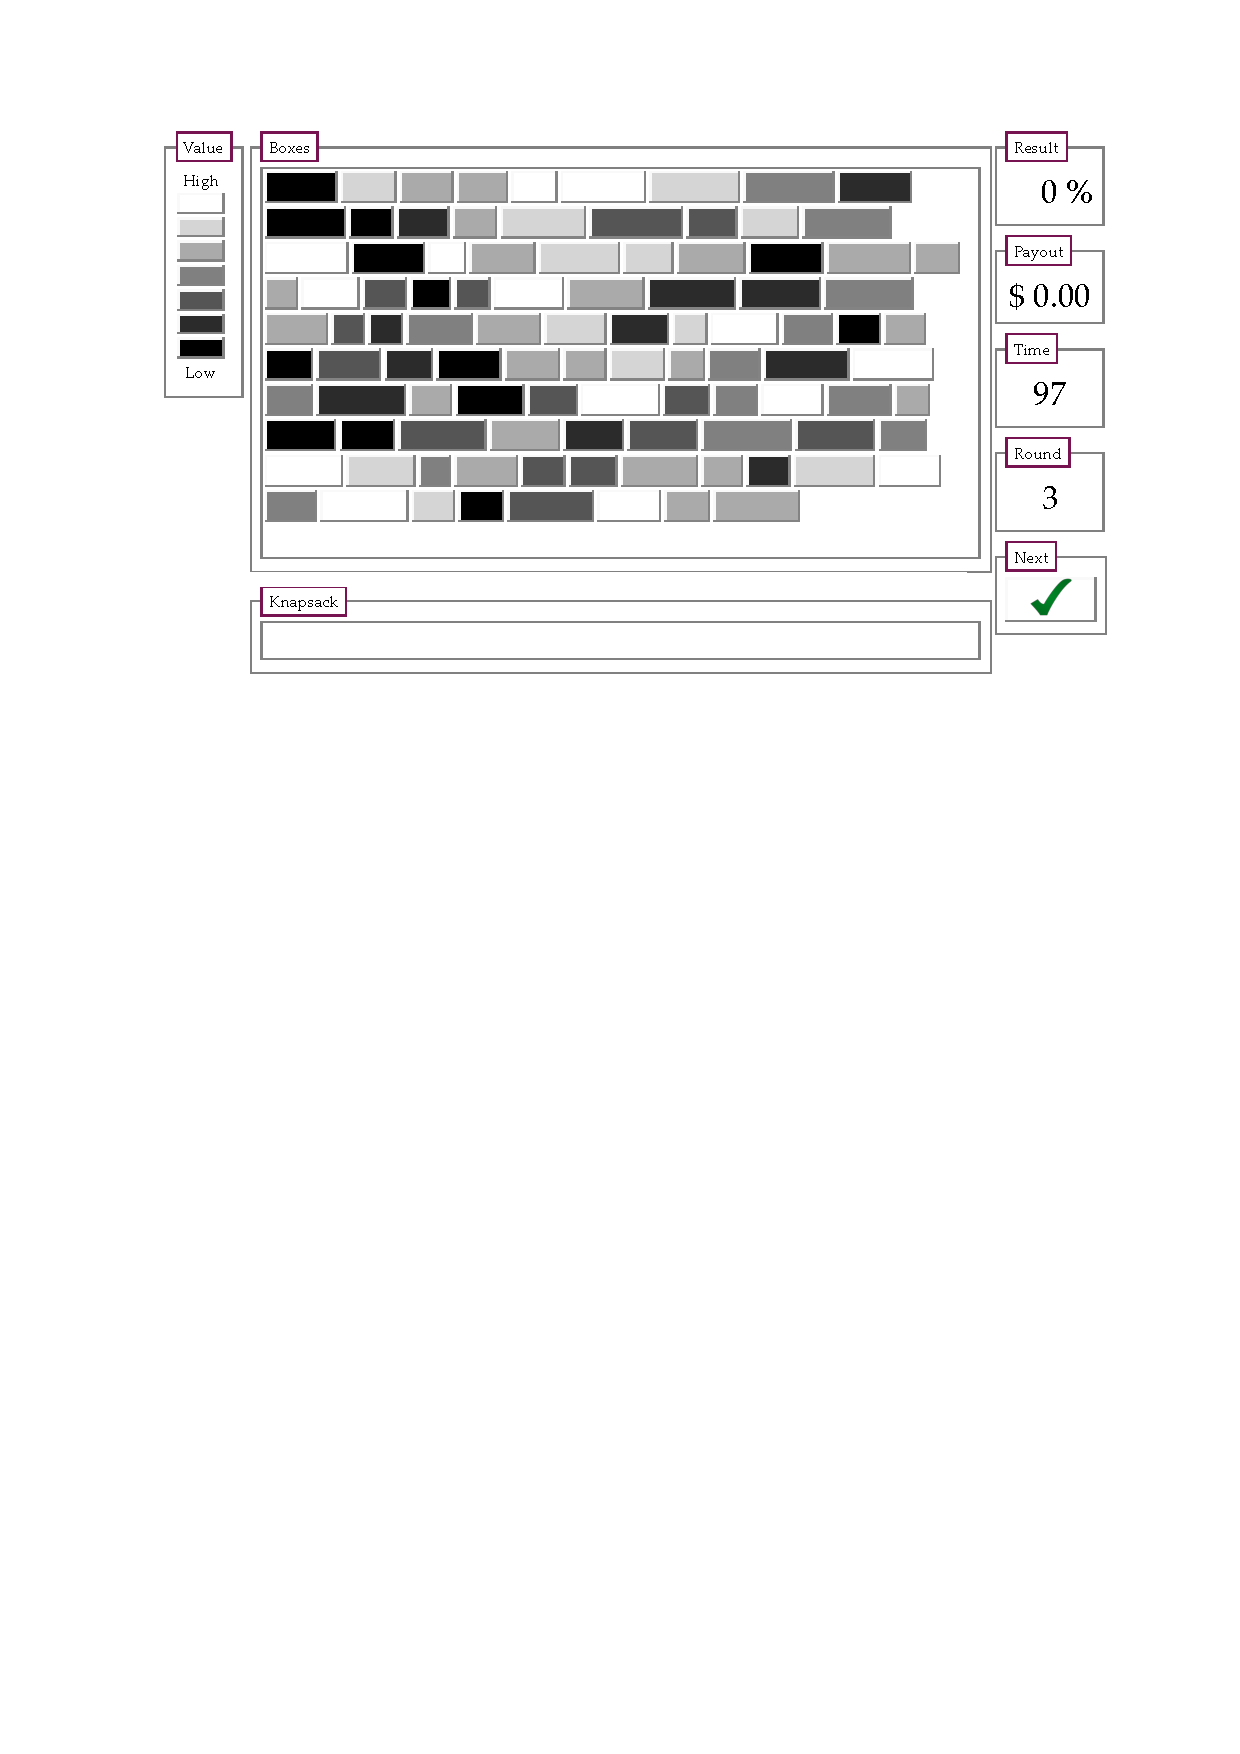
\includegraphics[height = 0.39\textwidth]{Interface2.pdf}
\end{subfigure}
\begin{subfigure} 
\centering
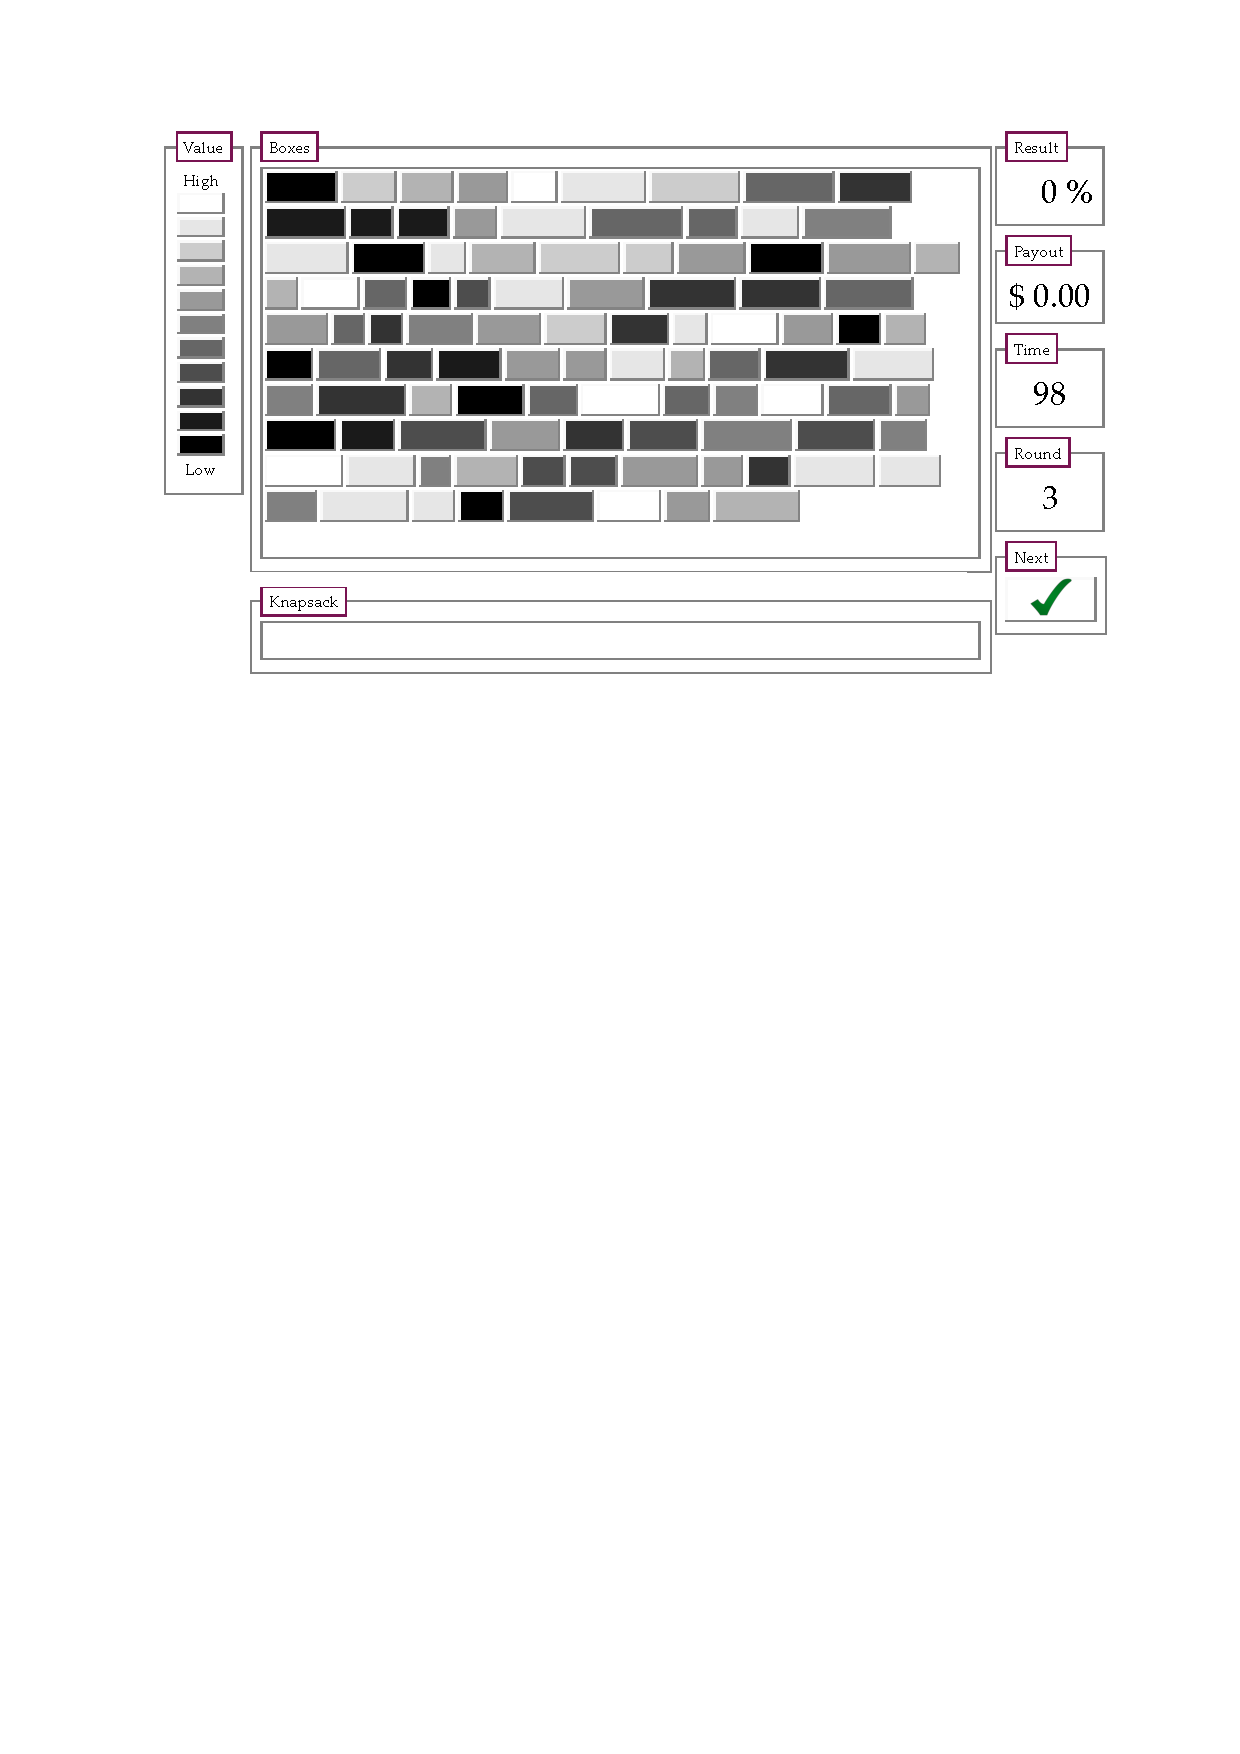
\includegraphics[height = 0.39\textwidth]{Interface3.pdf}
\end{subfigure}
  \caption{Interface for Usergroup 1, 2  and 3}
    \label{InterfaceOverview} 
\end{center}
\end{figure}

\newpage

\section{Formulas}
		\label{Appendix-Formulas}

%\begin{figure}[htbp]
%\begin{equation}
%\begin{split}
%x' = \dfrac{1}{4}x+\dfrac{1}{4},\;x = 3,7,11,15\quad \quad \quad\\ 
%x := number\;of\;colours,\;x' := new\;variable
%\end{split}
%\end{equation}
%\caption{Number of colours - Usergroup}
%\label{NumberUsergroup}
%\end{figure}
\begin{equation}
\begin{split}
Share\;of\;dropout = \dfrac{p_i(user|dropout)}{p_i(user)}, \quad \quad \\ 
i = 1,..4,\;user := number\;of\;users\;logged\;in
\end{split}
\end{equation}

\begin{equation}
\begin{split}
Share\;of\;minimum\;payout = \dfrac{p_i(user|payout=0)}{p_i(user)}, \\ 
i = 1,..4, user := number\;of\;users \quad \quad
\end{split}
\end{equation}

\begin{figure}[htbp]
\caption{Box - Cox - Transformation}
\label{BoxCoxTransformation}
\begin{equation}
y_i^{(\lambda)} = \begin{cases}
\dfrac{y_i^{\lambda}-1}{\lambda}, \quad if \lambda \neq 0, \\ 
log(y_i), \quad if \lambda = 0
\end{cases}, \quad y > 0 
\end{equation}

\end{figure}

\section{Descriptive statistics}
		\label{Appendix-Descriptive}
		
\begin{figure}[htbp] % DistributionFirstResult
\begin{center} 
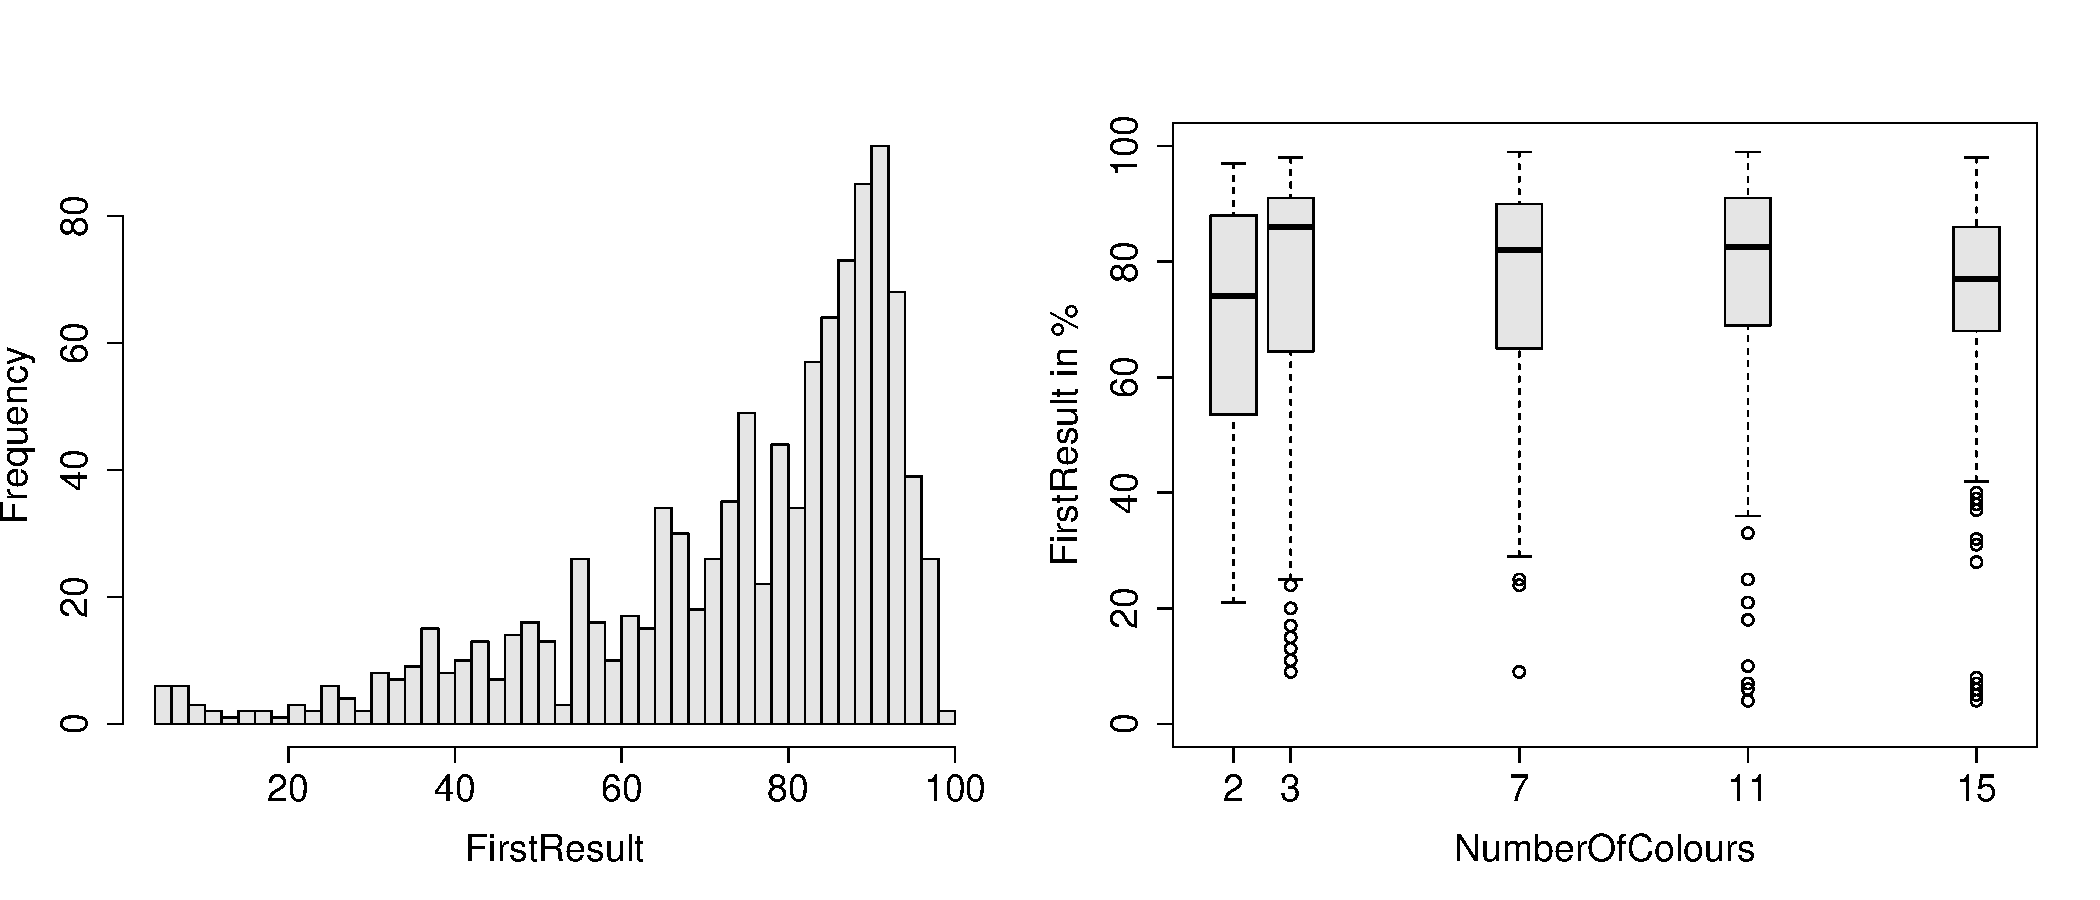
\includegraphics[height = 0.38\textwidth]{DescriptivesFirstResult.pdf}
  \caption{FirstResult - Histogram and Box plot}
    \label{DistributionFirstResult} 
\end{center}
\end{figure}

\begin{figure}[htbp] % DistributionBestResult
\begin{center} 
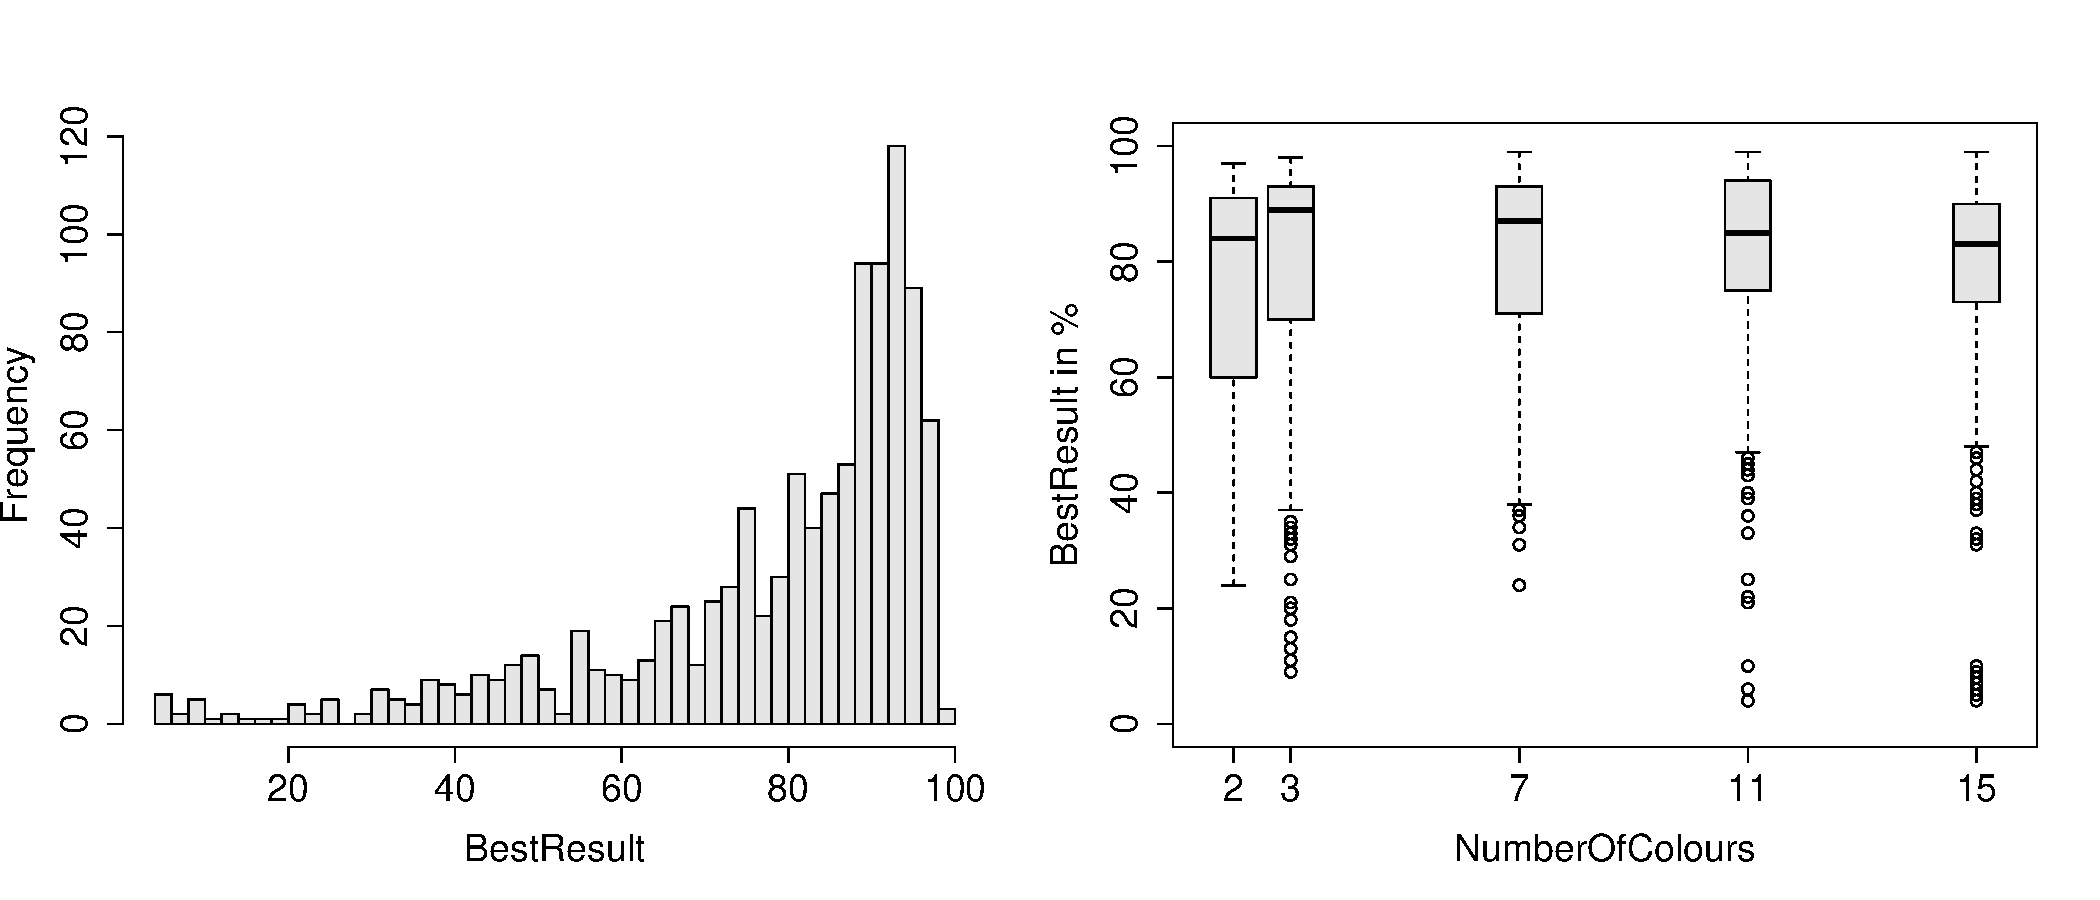
\includegraphics[height = 0.38\textwidth]{DescriptivesBestResult.pdf}
  \caption{BestResult - Histogram and Box plot}
    \label{DistributionBestResult} 
\end{center}
\end{figure}

\begin{figure}[htbp] % DistributionFirstTime
\begin{center} 
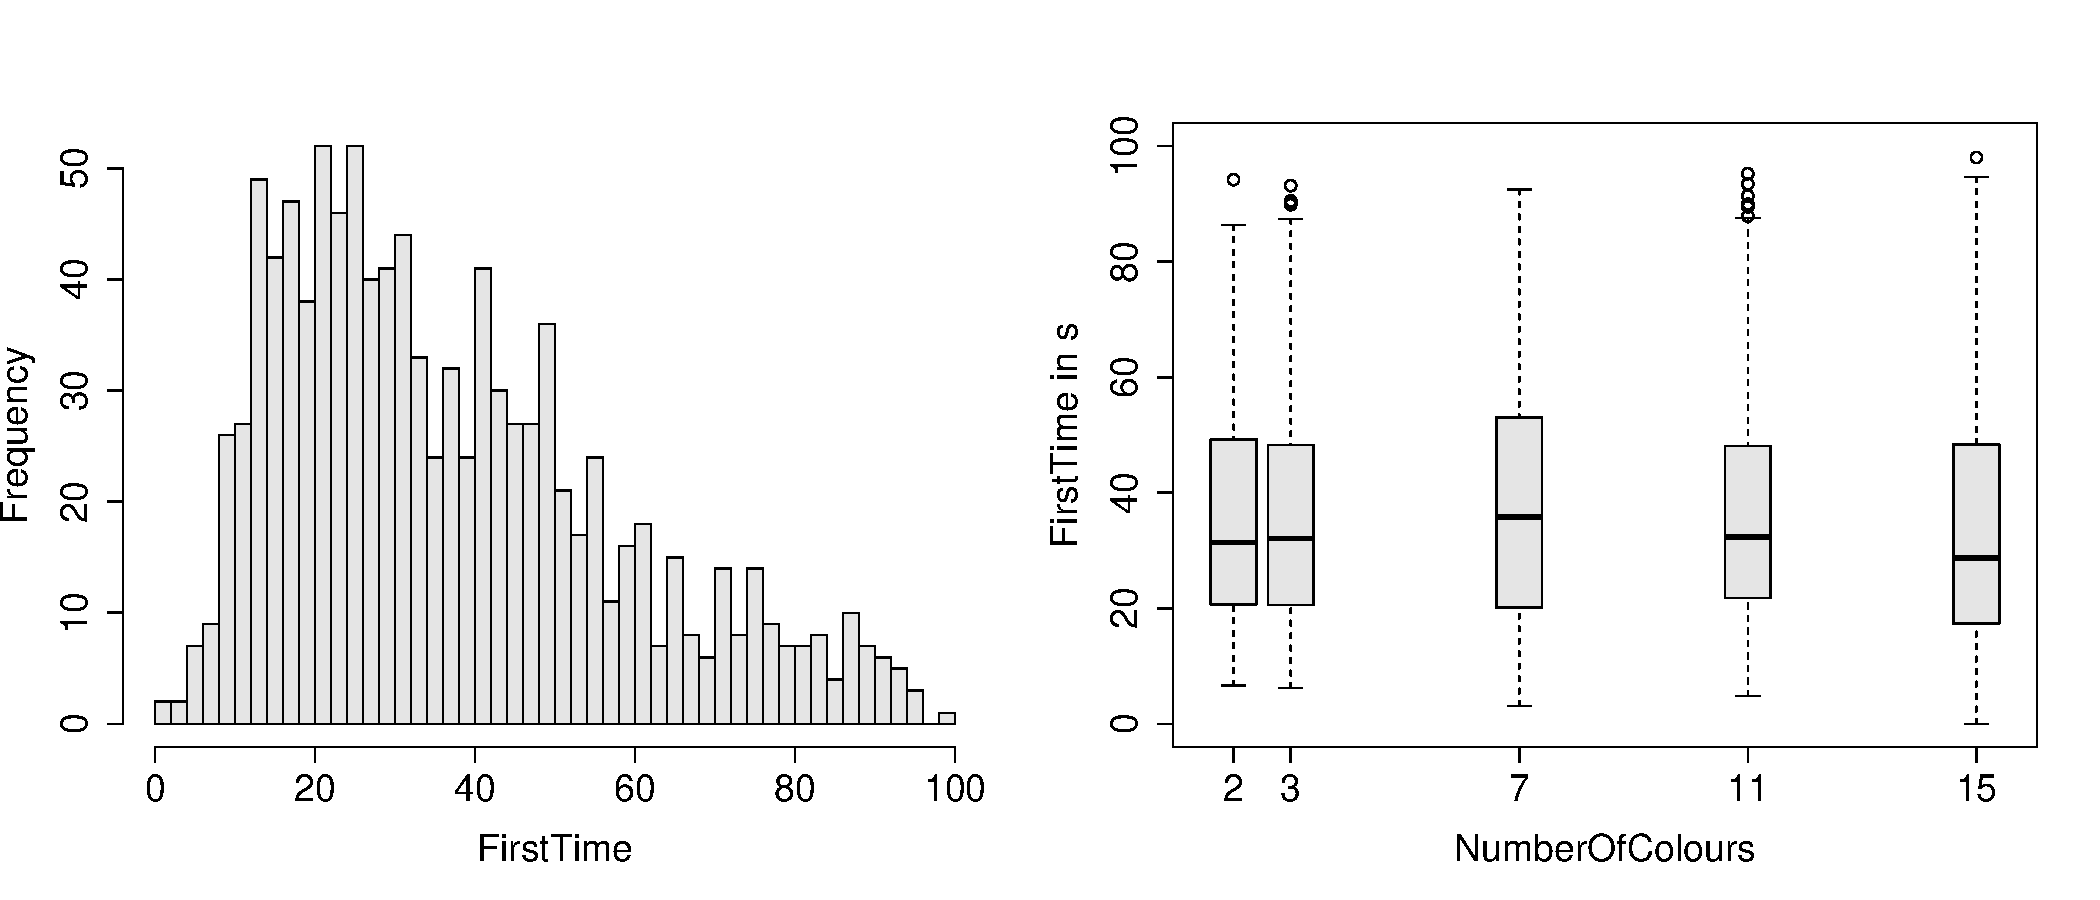
\includegraphics[height = 0.38\textwidth]{DescriptivesFirstTime.pdf}
  \caption{FirstTime - Histogram and Box plot}
    \label{DistributionFirstTime} 
\end{center}
\end{figure}
\begin{figure}[htbp] % DistributionBestTime
\begin{center} 
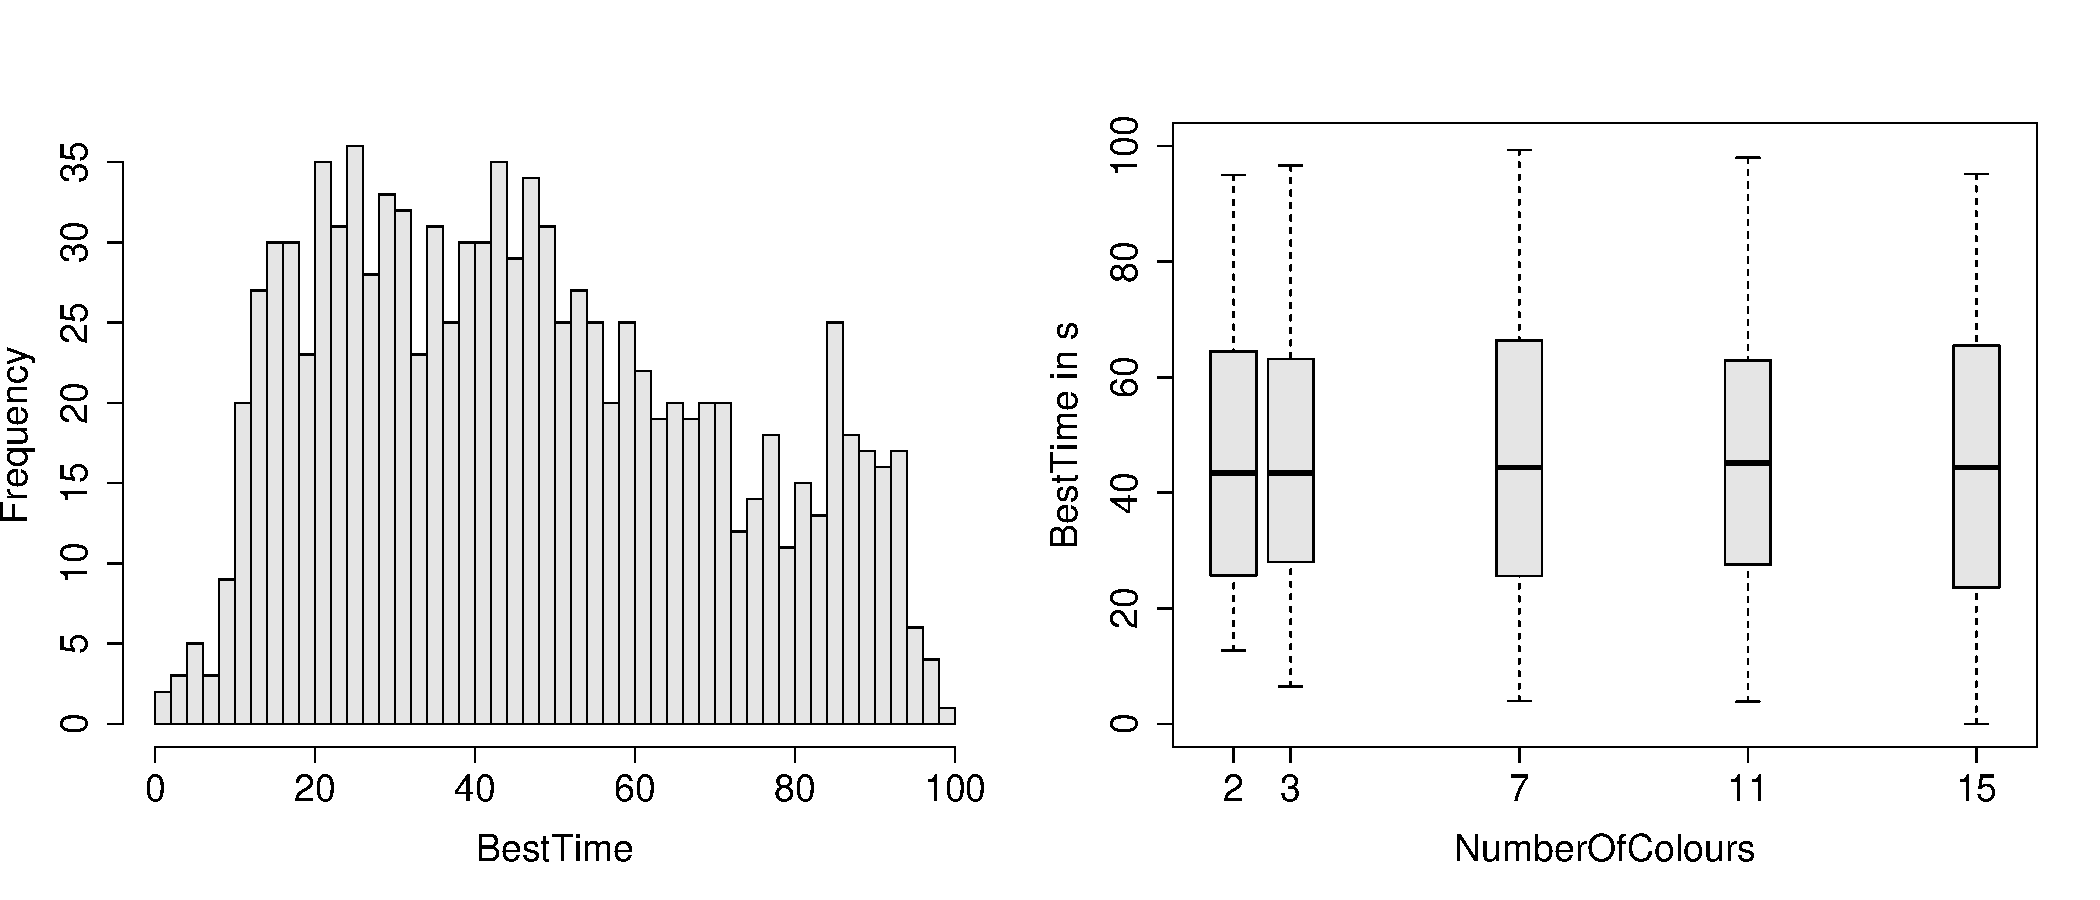
\includegraphics[height = 0.38\textwidth]{DescriptivesBestTime.pdf}
  \caption{BestTime - Histogram and Box plot}
    \label{DistributionBestTime} 
\end{center}
\end{figure}

\begin{figure}[htbp] % DistributionDecisionTime
\begin{center} 
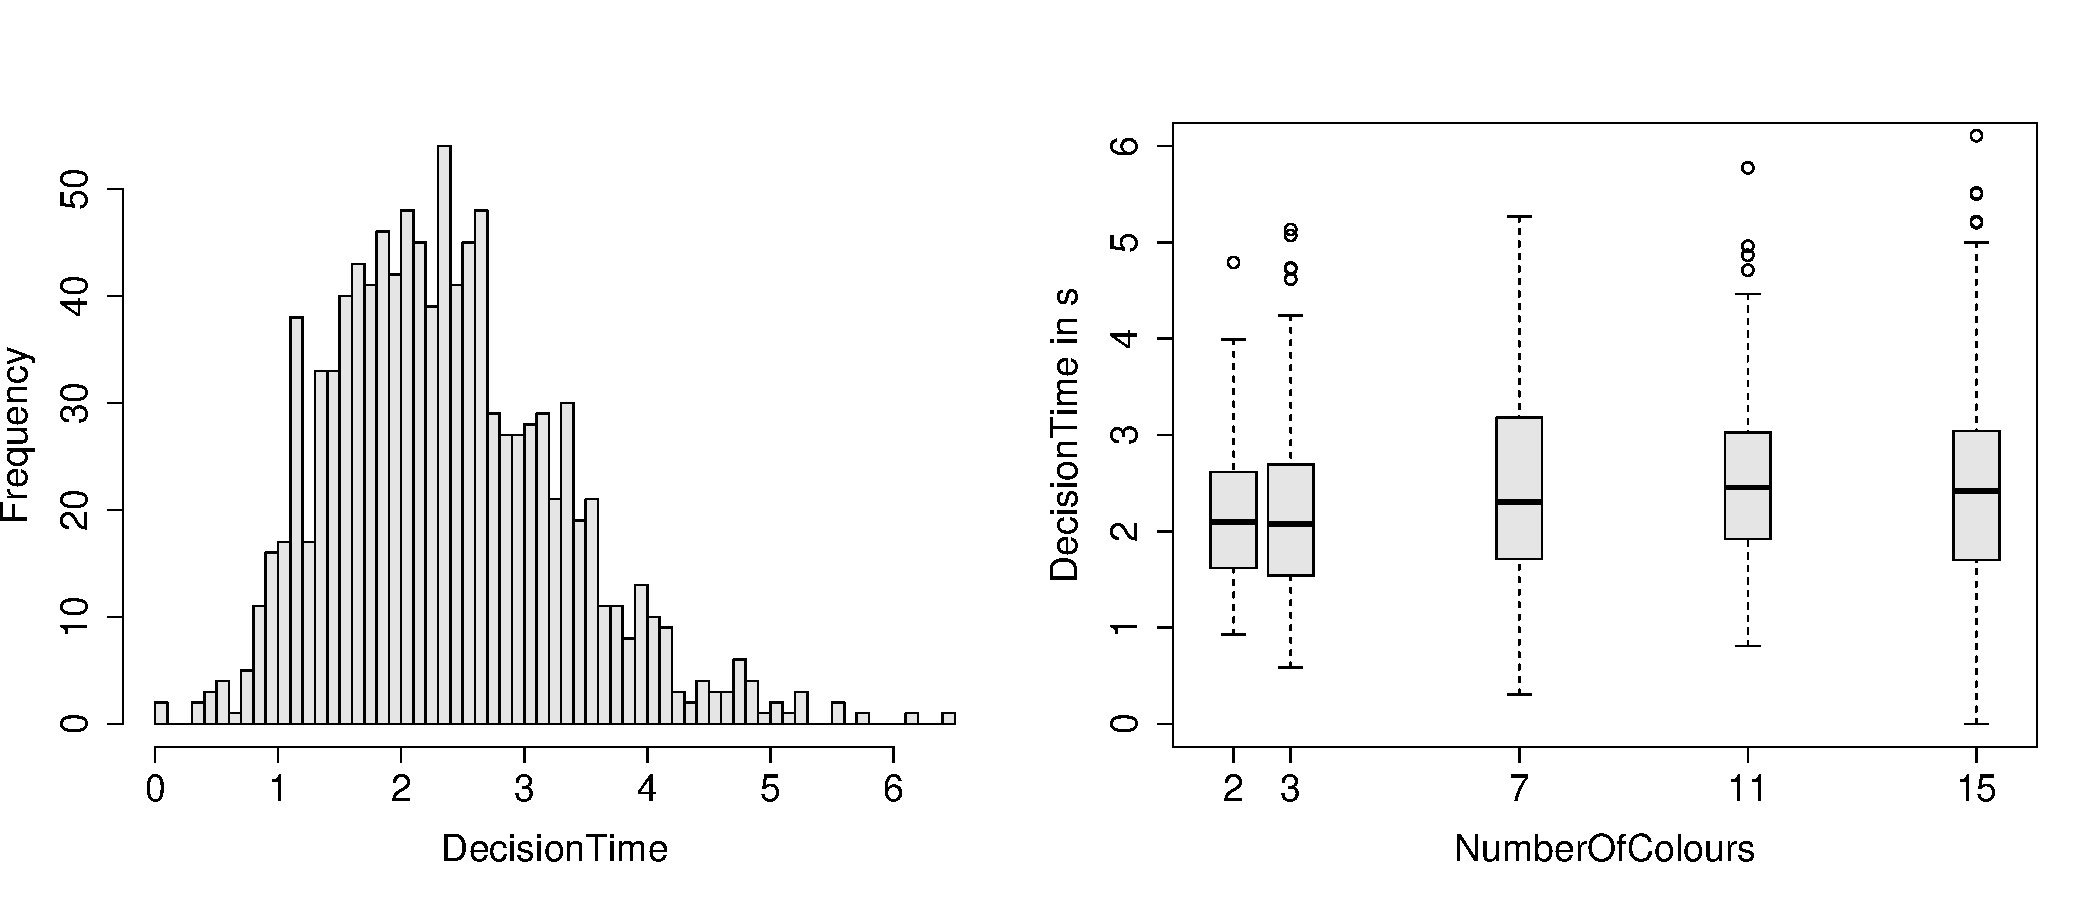
\includegraphics[height = 0.38\textwidth]{DescriptivesDecisionTime.pdf}
  \caption{DecisionTime - Histogram and Box plot}
    \label{DistributionDecisionTime} 
\end{center}
\end{figure}

\begin{figure}[!ht] % Question1
\centering
  \caption[Question 1 - Histogram and Box plot]{Question 1 - very low (1) to very high (7)}
    \label{Question1}  
\begin{subfigure} 
\centering
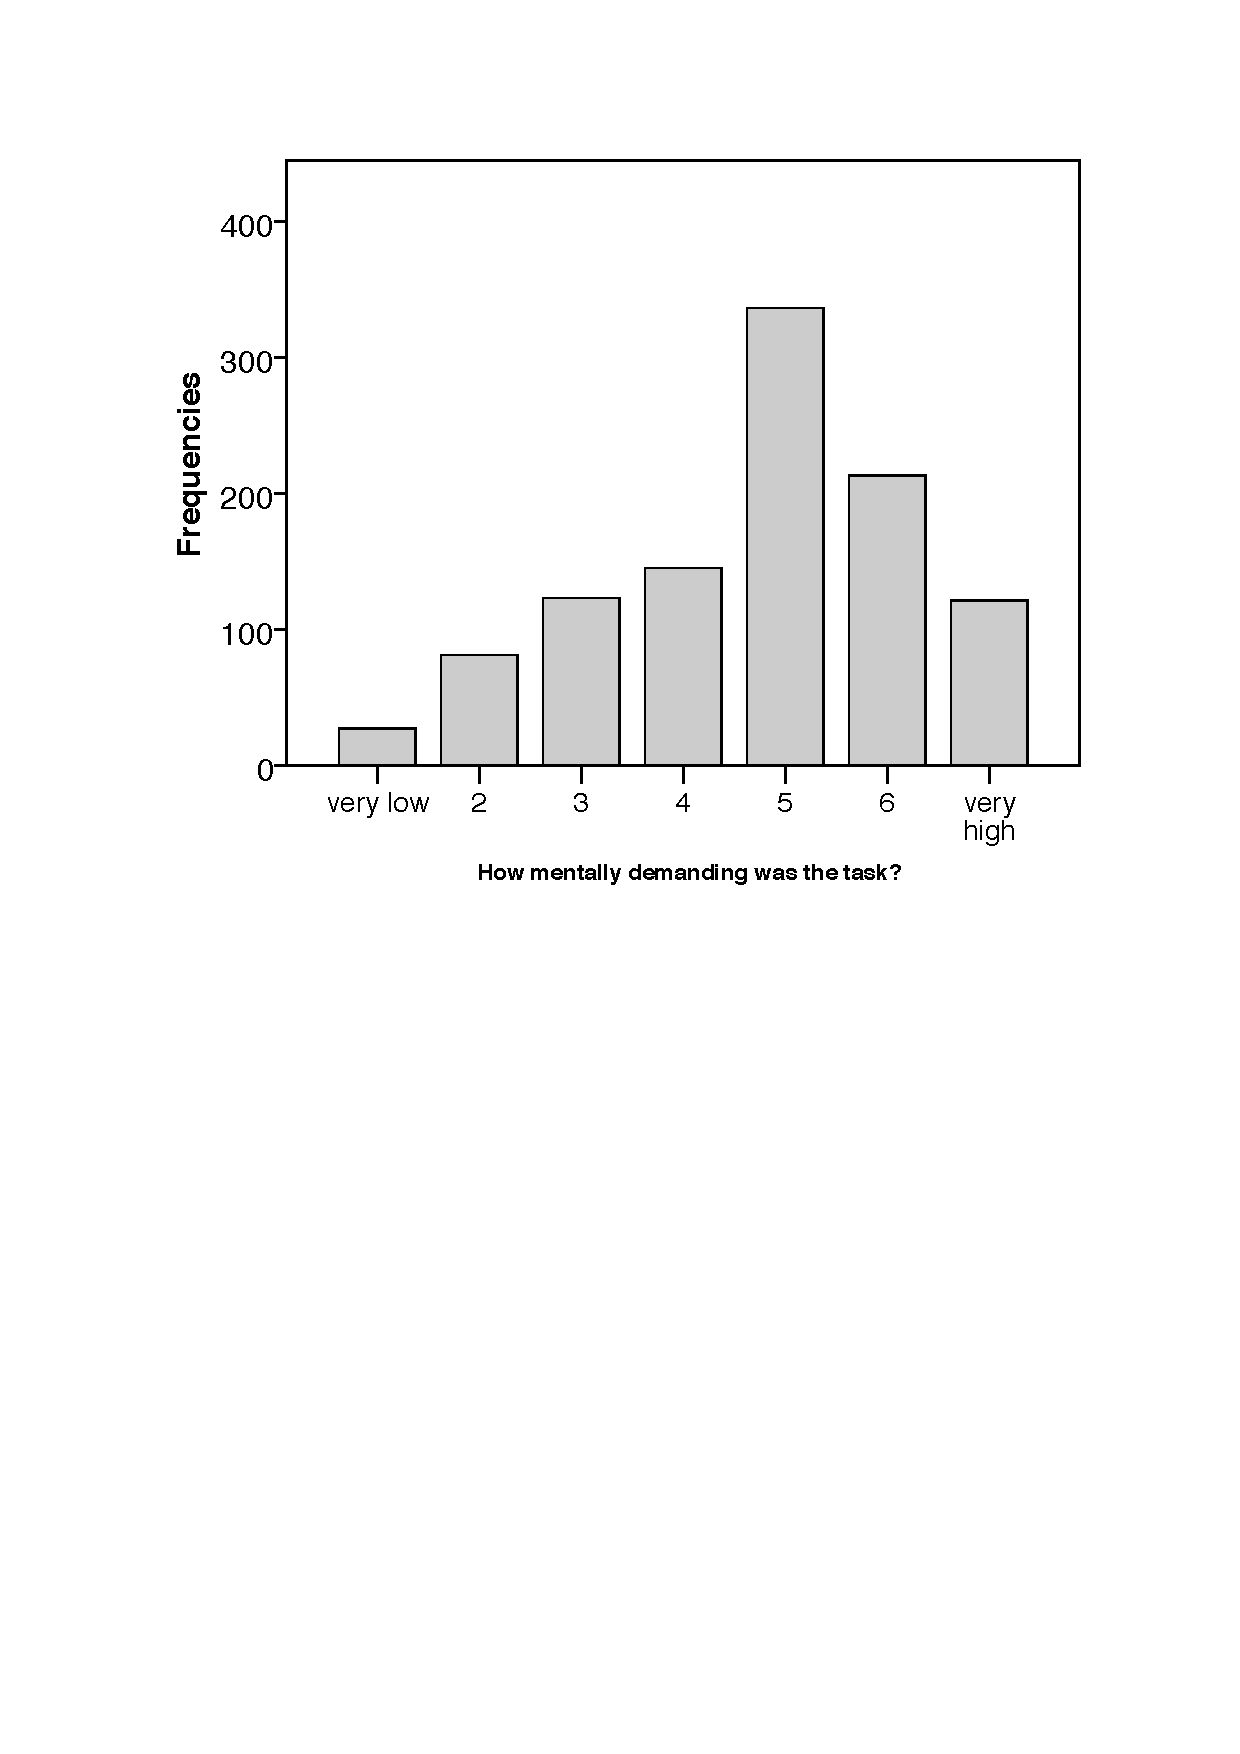
\includegraphics[height = 0.38\textwidth]{HistogramQuestion1.pdf}
\end{subfigure} 
\begin{subfigure} 
\centering
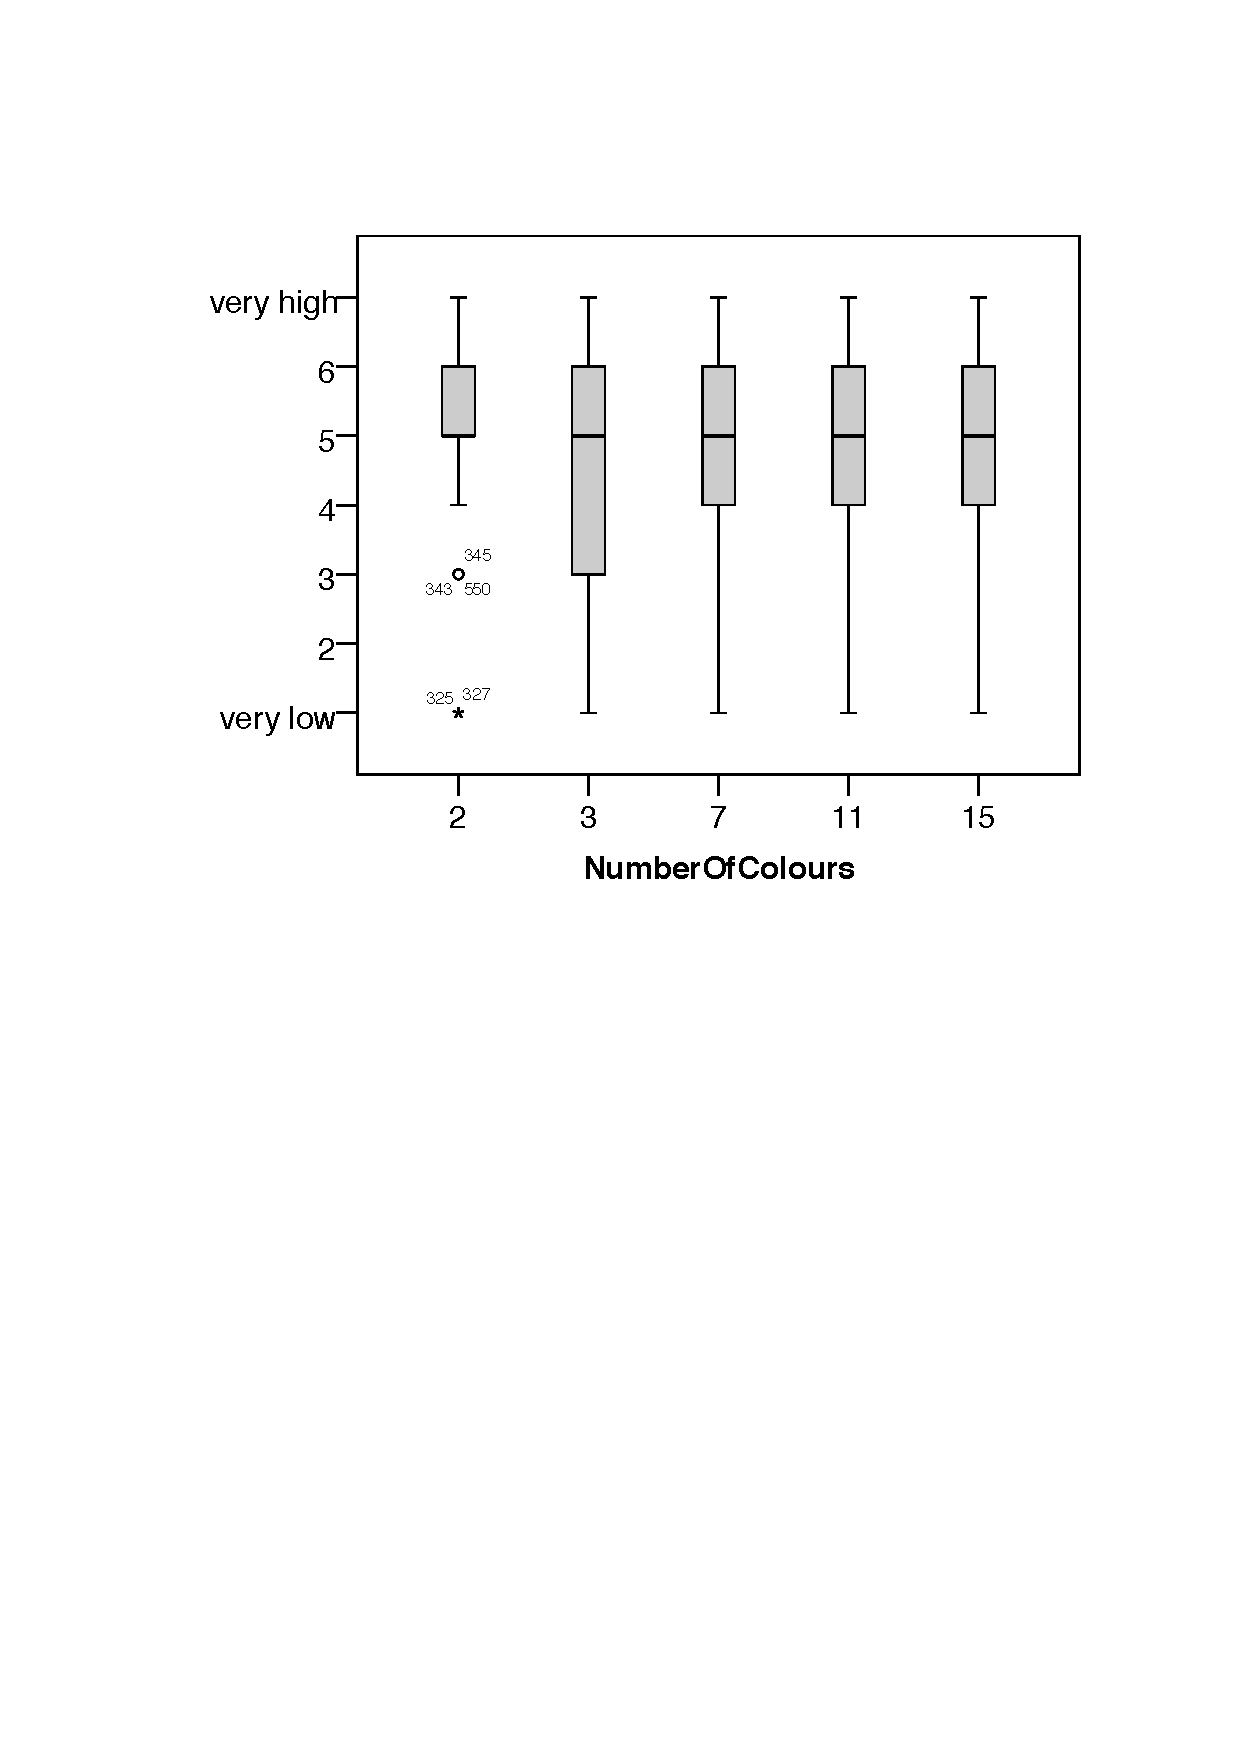
\includegraphics[height = 0.38\textwidth]{BoxplotQuestion1.pdf}
\end{subfigure}
\end{figure}
\begin{figure}[H] % Question2	
\begin{center} 
\begin{subfigure} 
\centering
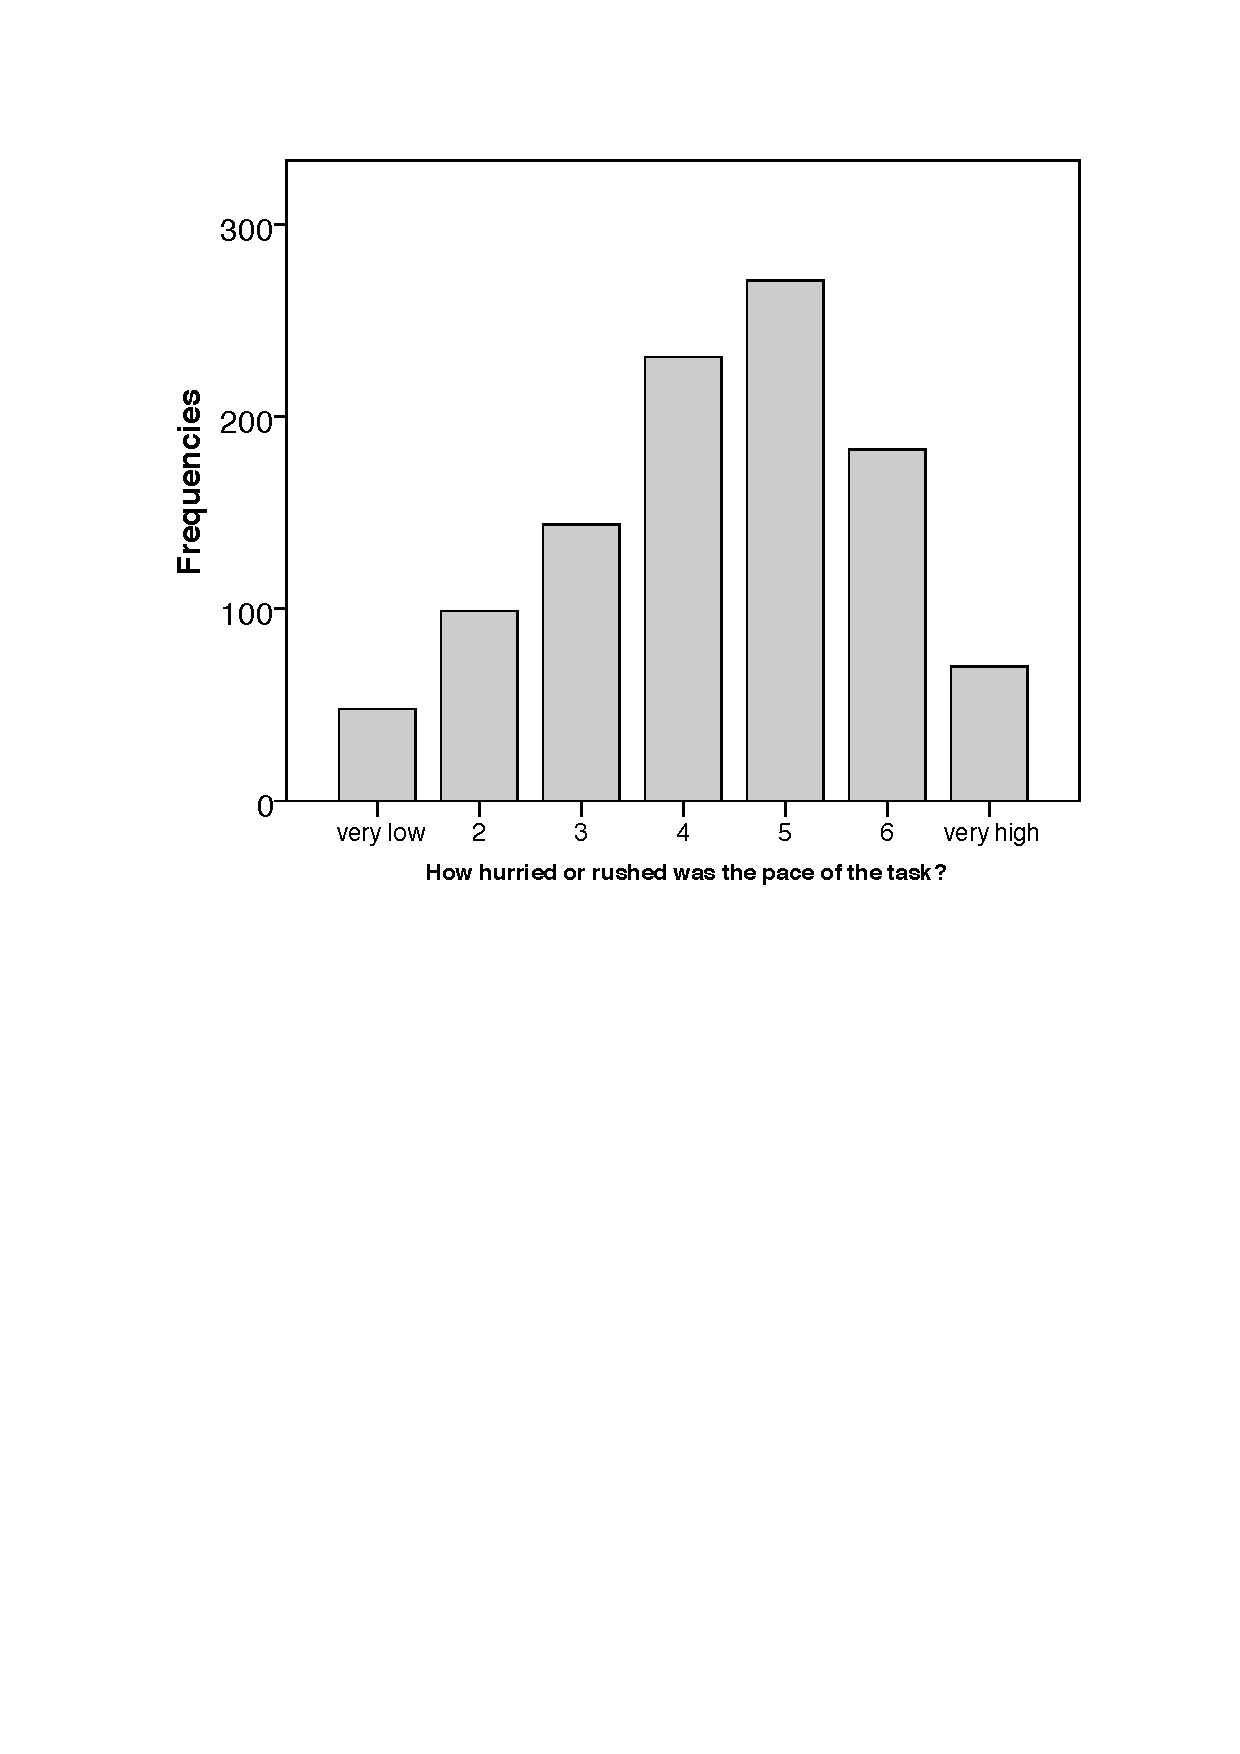
\includegraphics[height = 0.38\textwidth]{HistogramQuestion2.pdf}
\end{subfigure} 
\begin{subfigure} 
\centering
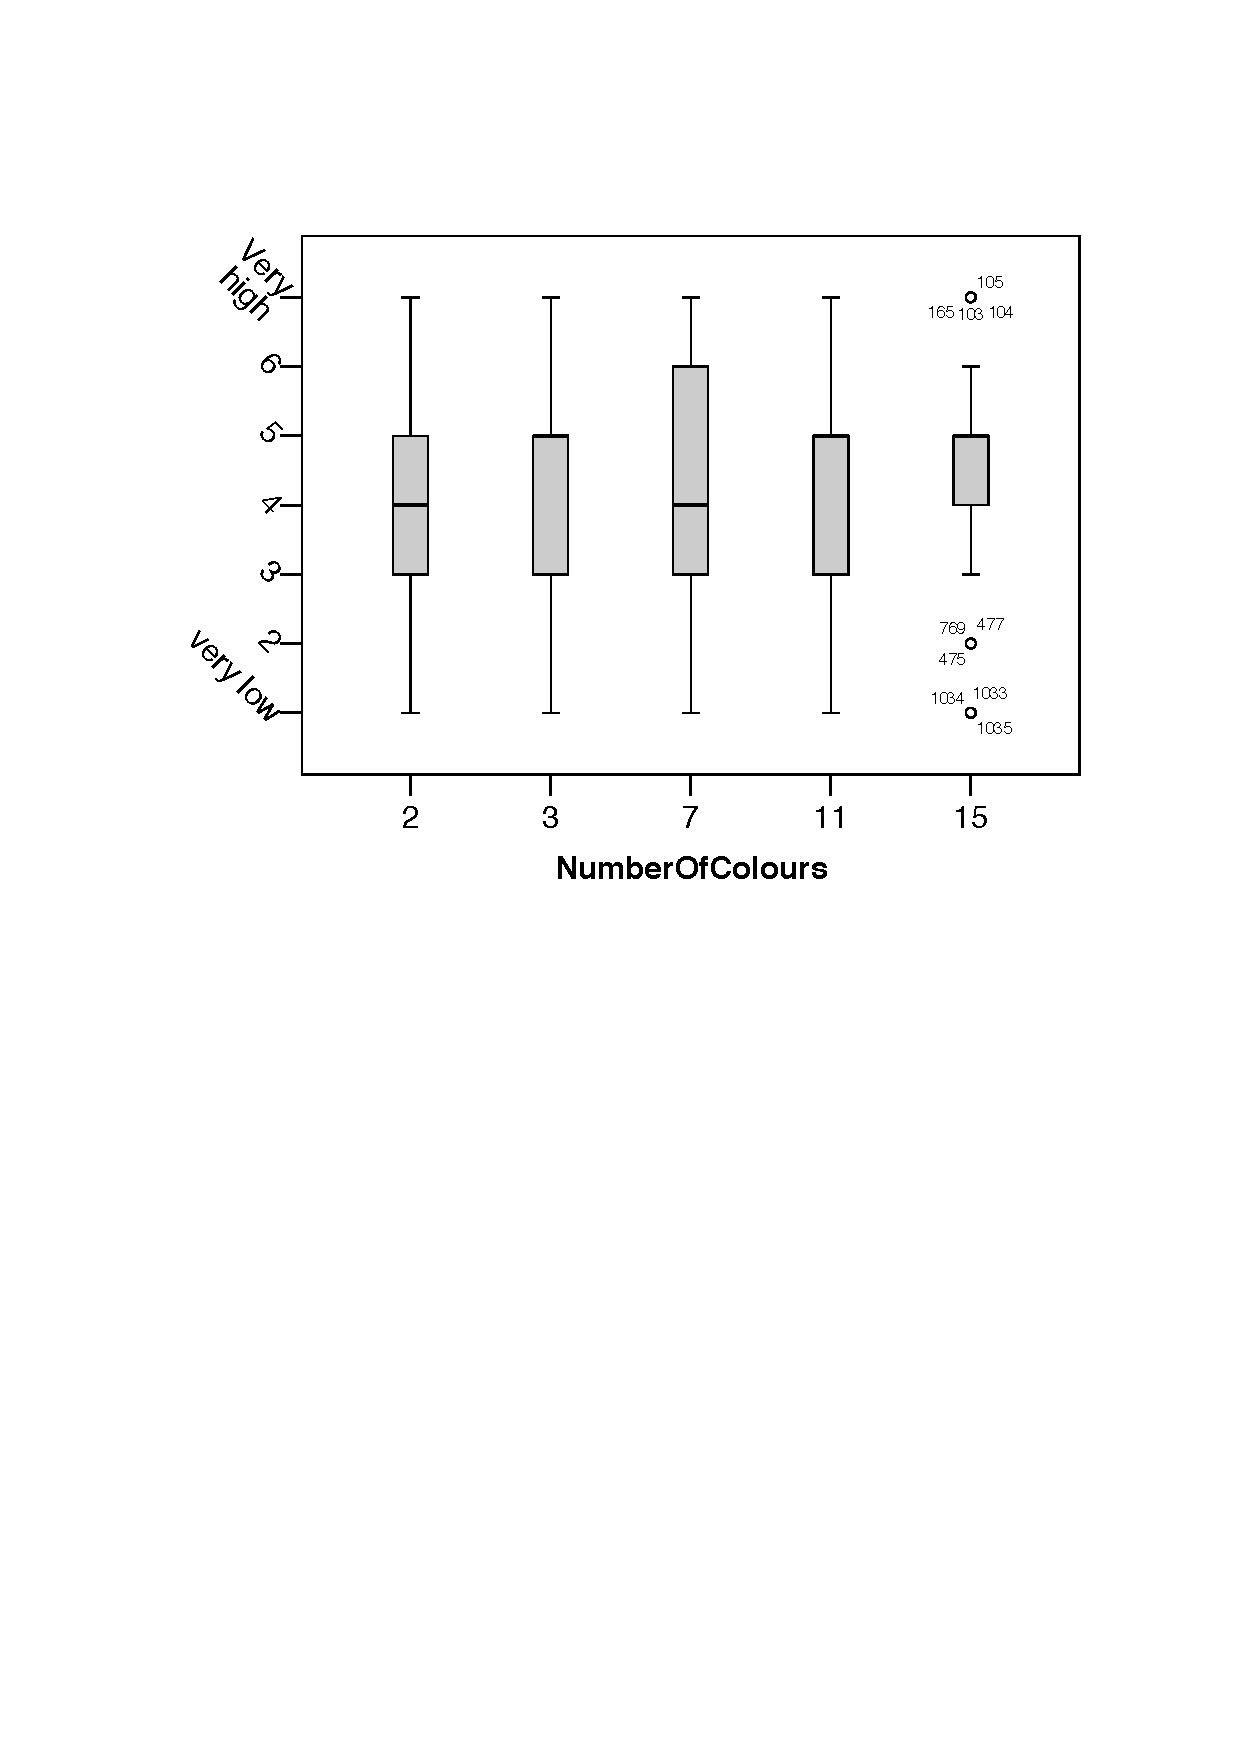
\includegraphics[height = 0.38\textwidth]{BoxplotQuestion2.pdf}
\end{subfigure}
  \caption[Question 2 - Histogram and Box plot]{Question 2 - very low (1) to very high (7)}
    \label{Question2} 
\end{center}
\end{figure}
\begin{figure}[htbp] % Question3	
\begin{center} 
\begin{subfigure} 
\centering
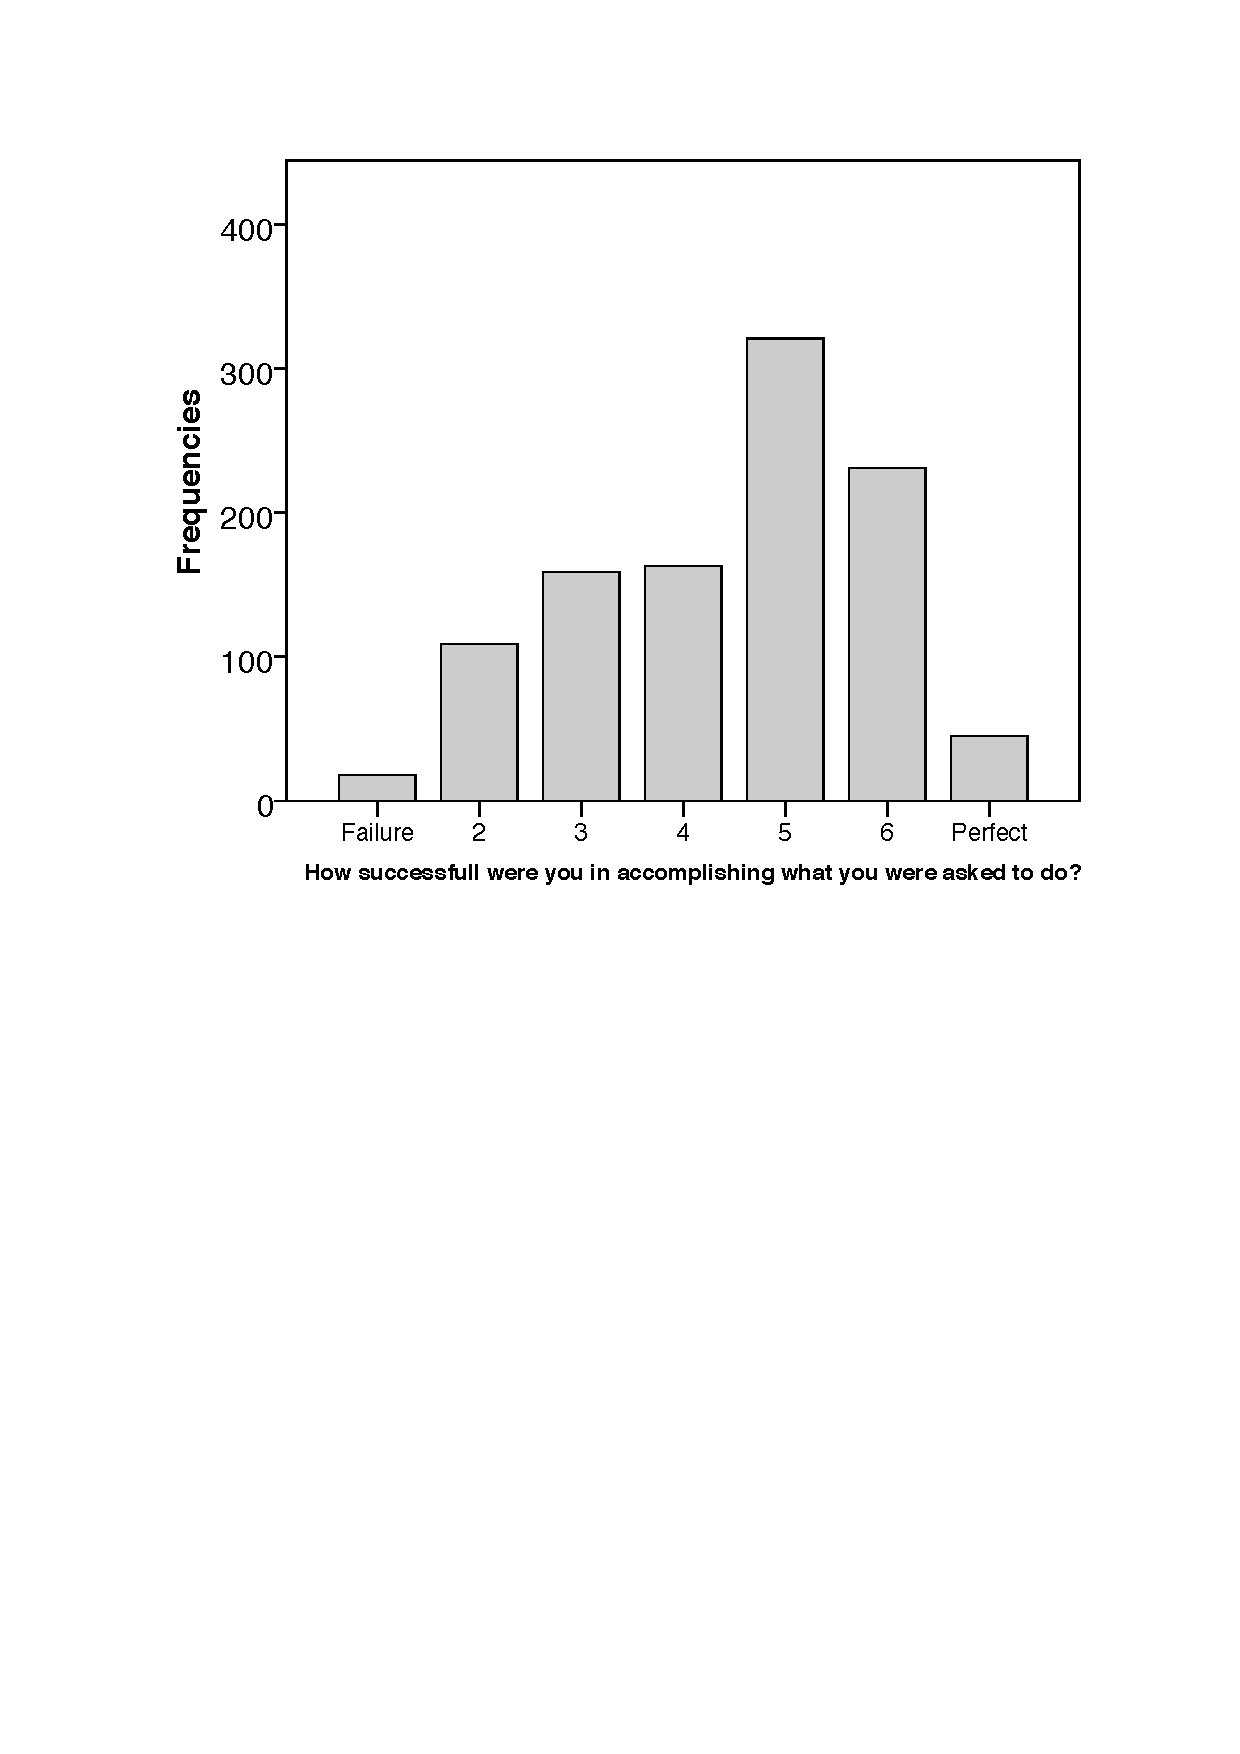
\includegraphics[height = 0.35\textwidth]{HistogramQuestion3.pdf}
\end{subfigure} 
\begin{subfigure} 
\centering
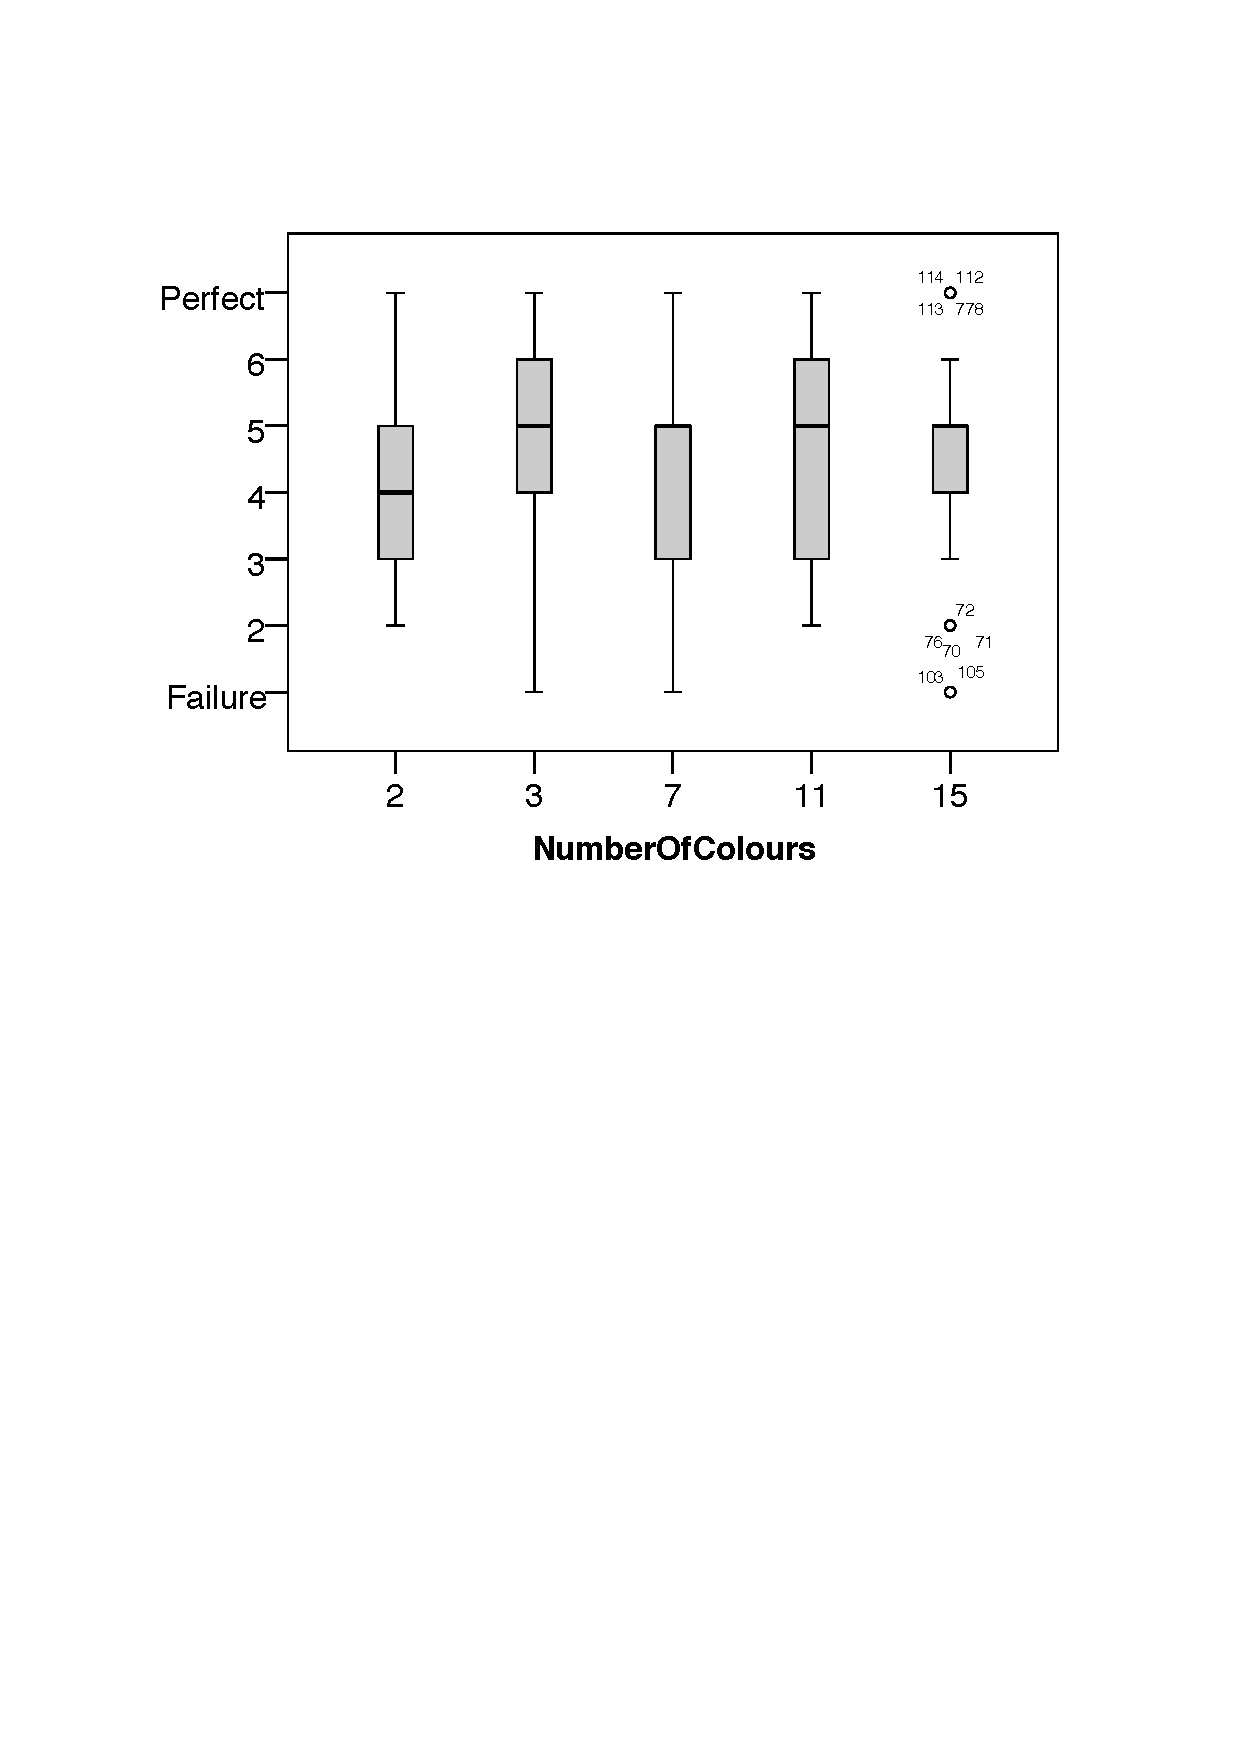
\includegraphics[height = 0.35\textwidth]{BoxplotQuestion3.pdf}
\end{subfigure}
  \caption[Question 3 - Histogram and Box plot]{Question 3 - Failure (1) to Perfect (7)}
    \label{Question3} 
\end{center}
\end{figure}
\begin{figure}[htbp] % Question4	
\begin{center} 
\begin{subfigure} 
\centering
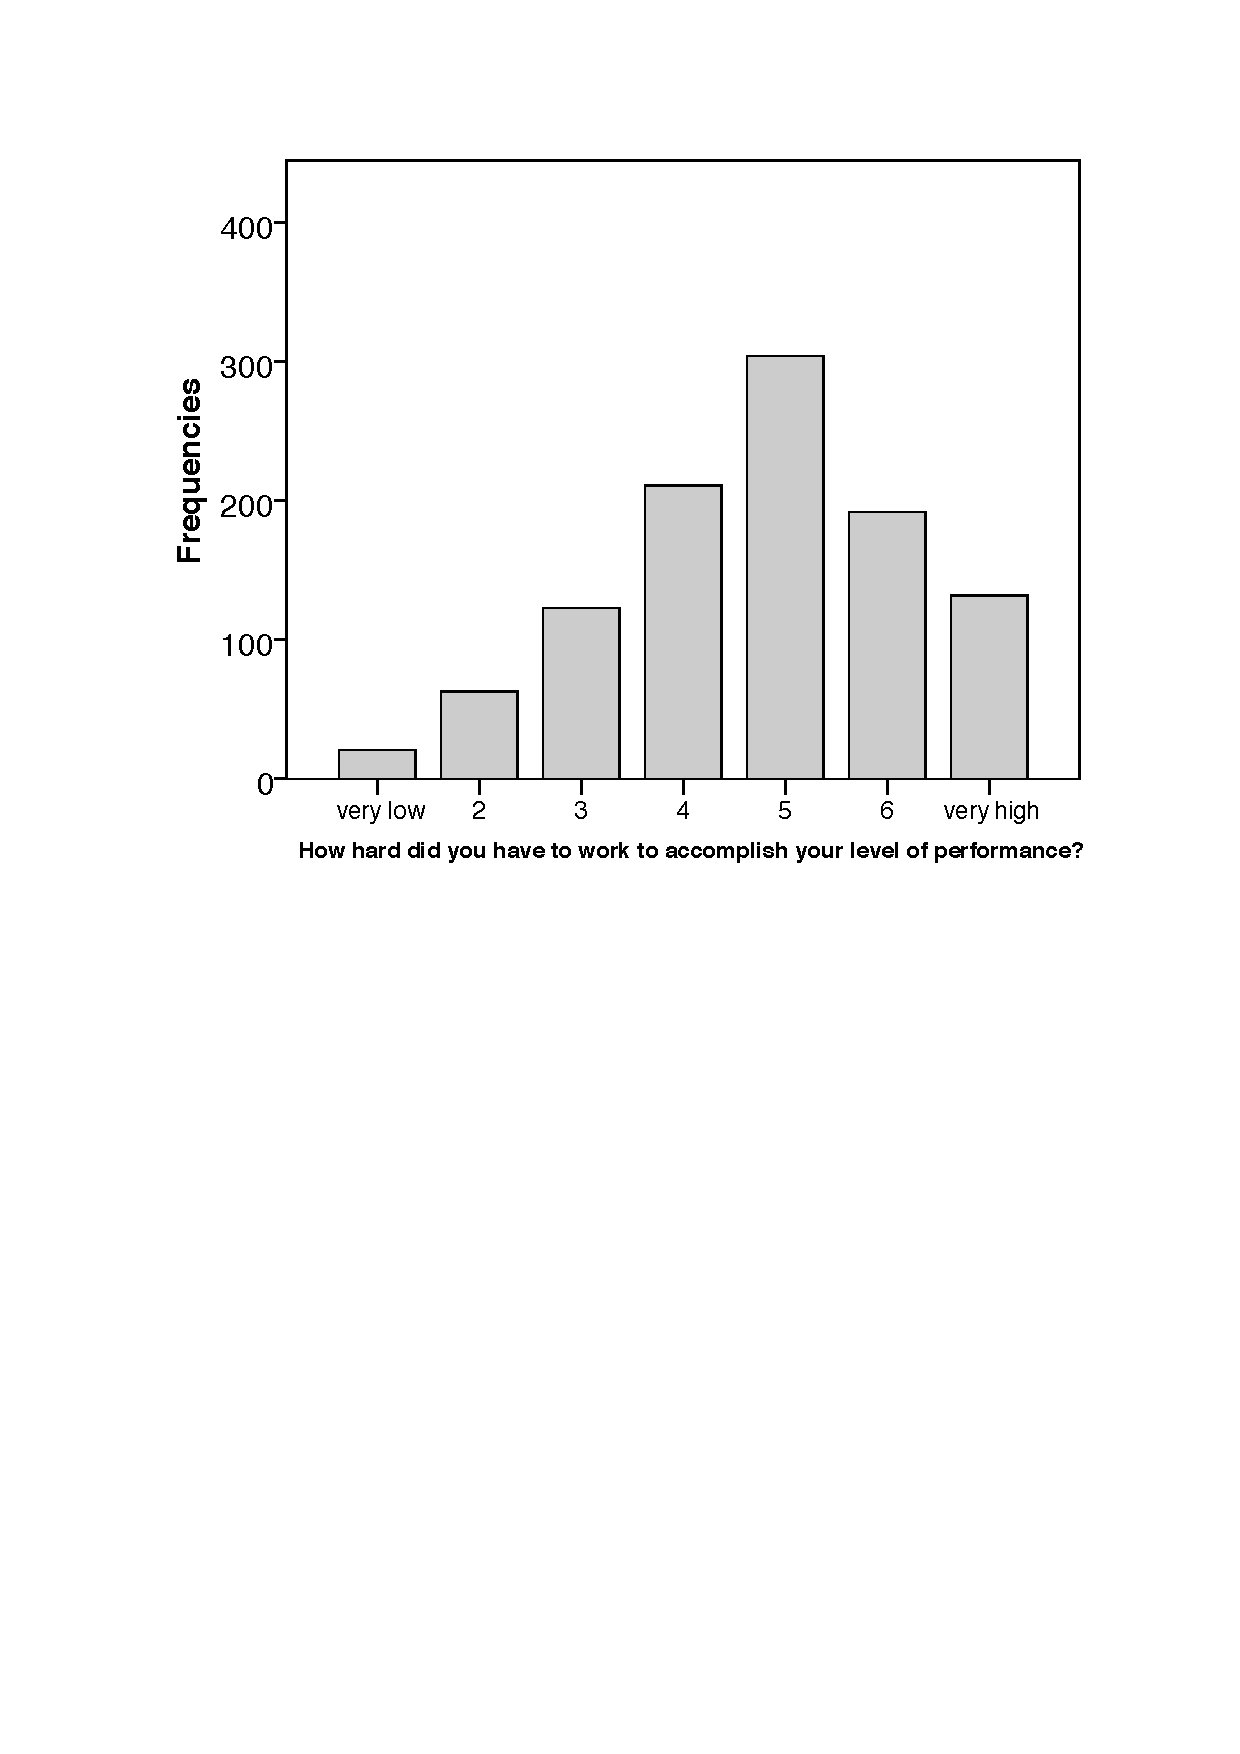
\includegraphics[height = 0.35\textwidth]{HistogramQuestion4.pdf}
\end{subfigure} 
\begin{subfigure} 
\centering
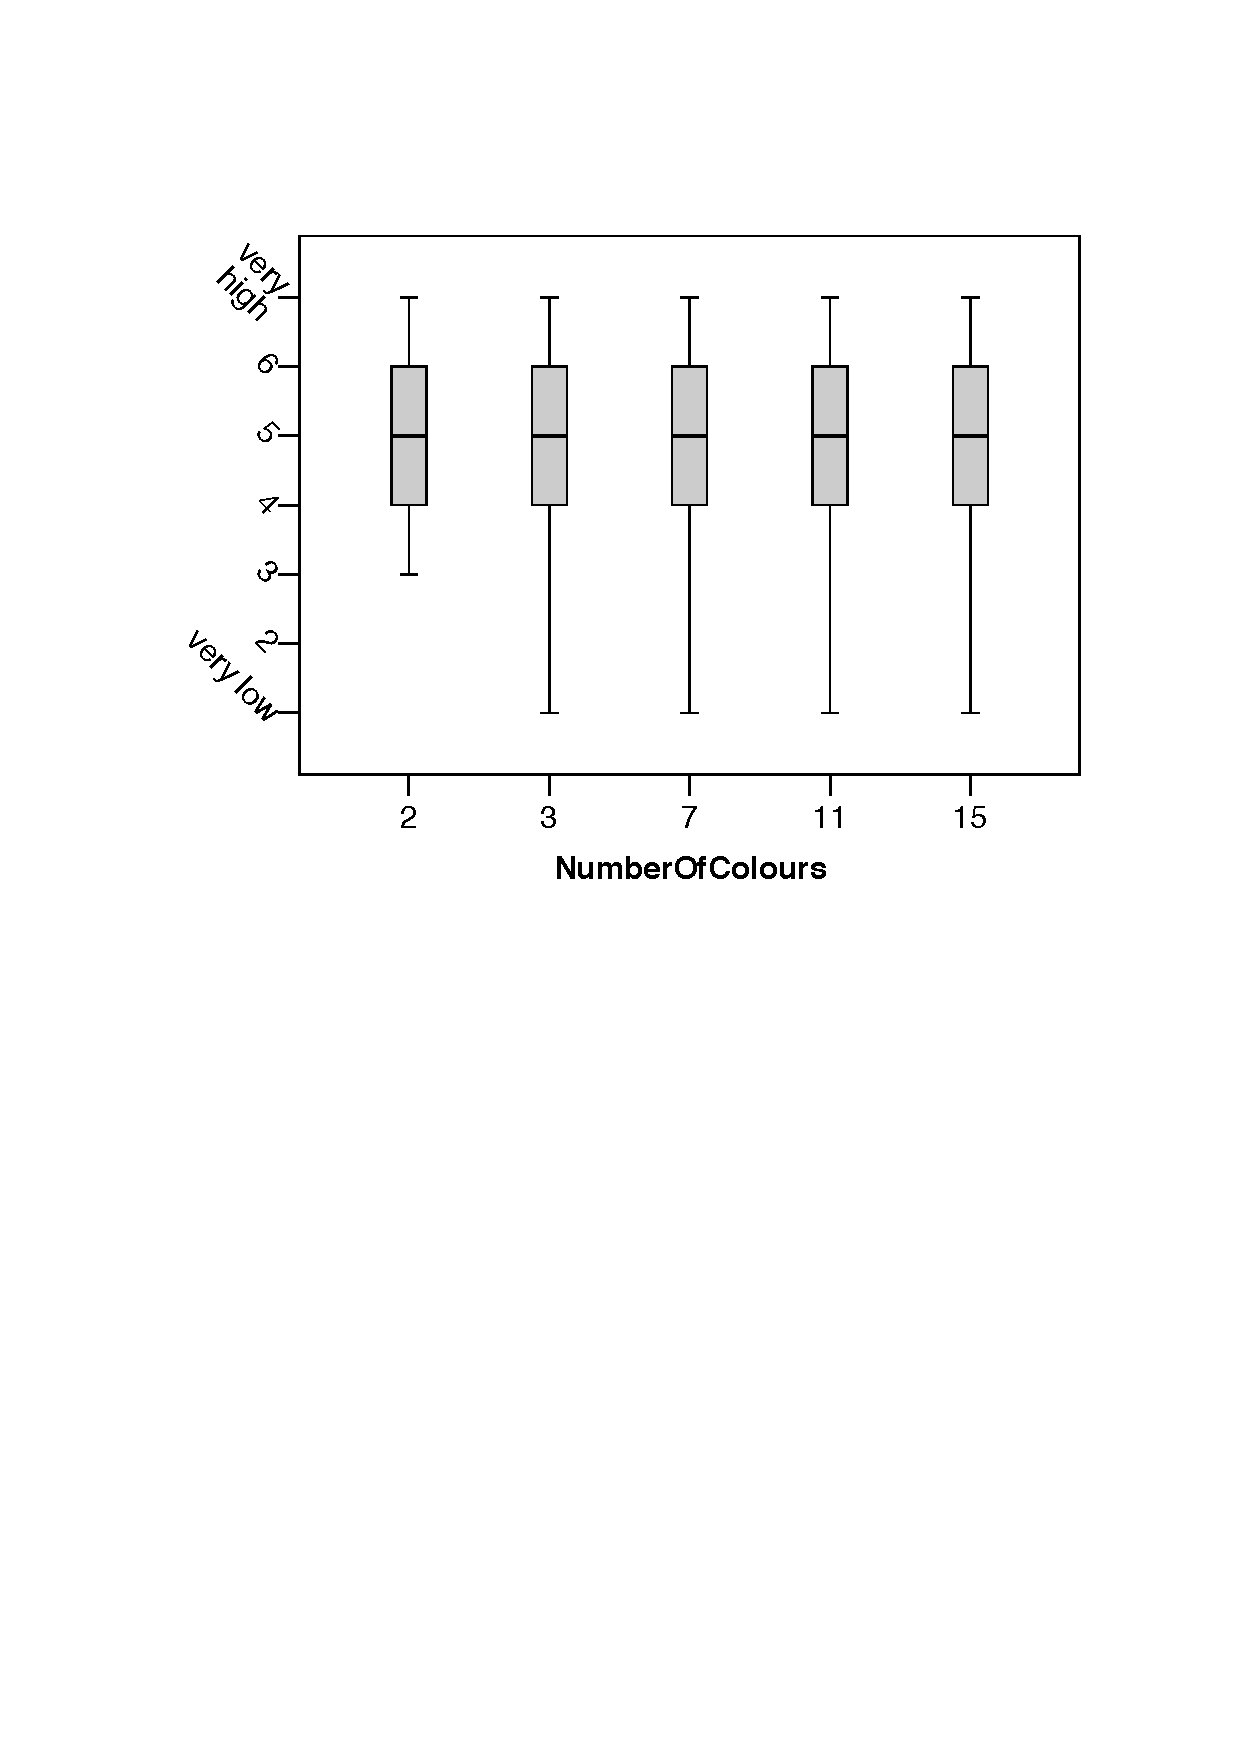
\includegraphics[height = 0.35\textwidth]{BoxplotQuestion4.pdf}
\end{subfigure}
  \caption[Question 4 - Histogram and Box plot]{Question 4 - very low (1) to very high (7}
    \label{Question4} 
\end{center}
\end{figure}
\begin{figure}[htbp] % Question5	
\begin{center} 
\begin{subfigure} 
\centering
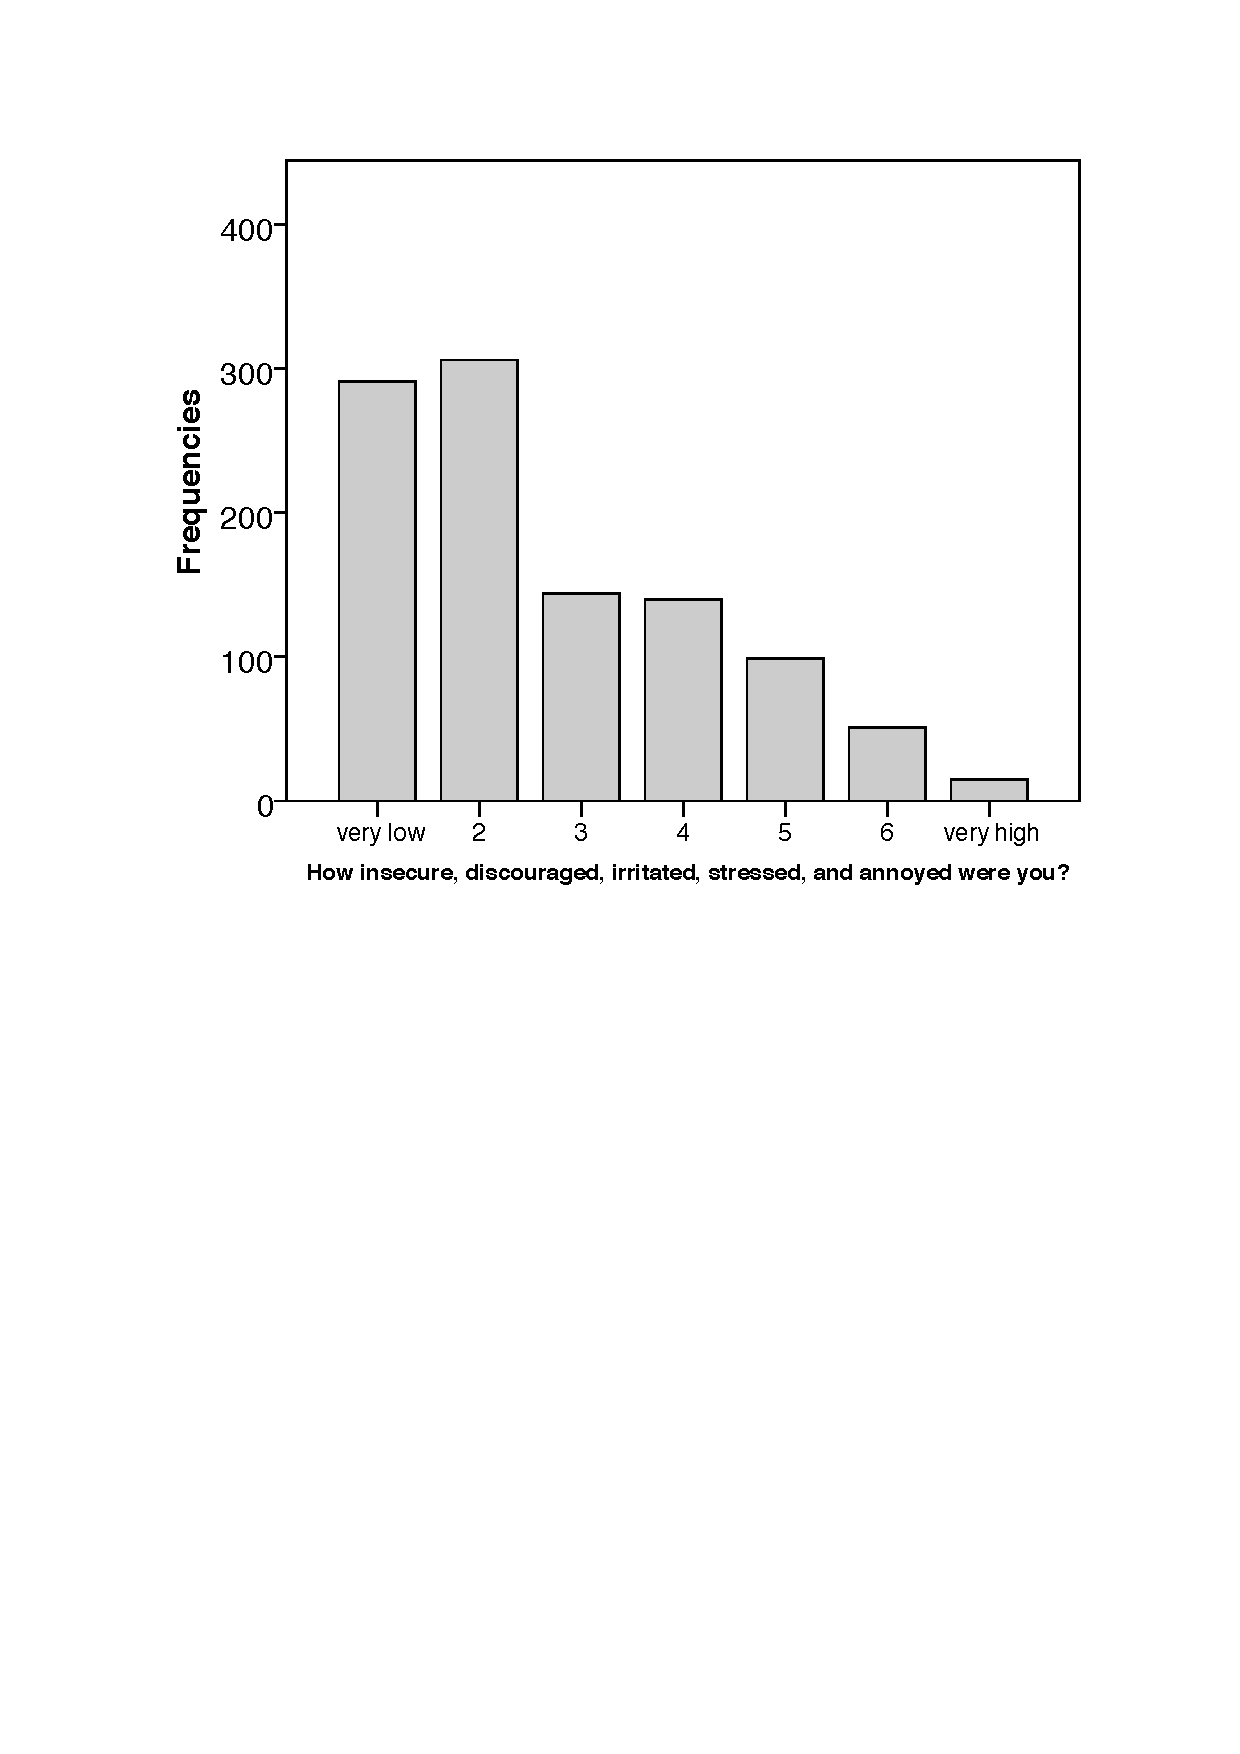
\includegraphics[height = 0.35\textwidth]{HistogramQuestion5.pdf}
\end{subfigure} 
\begin{subfigure} 
\centering
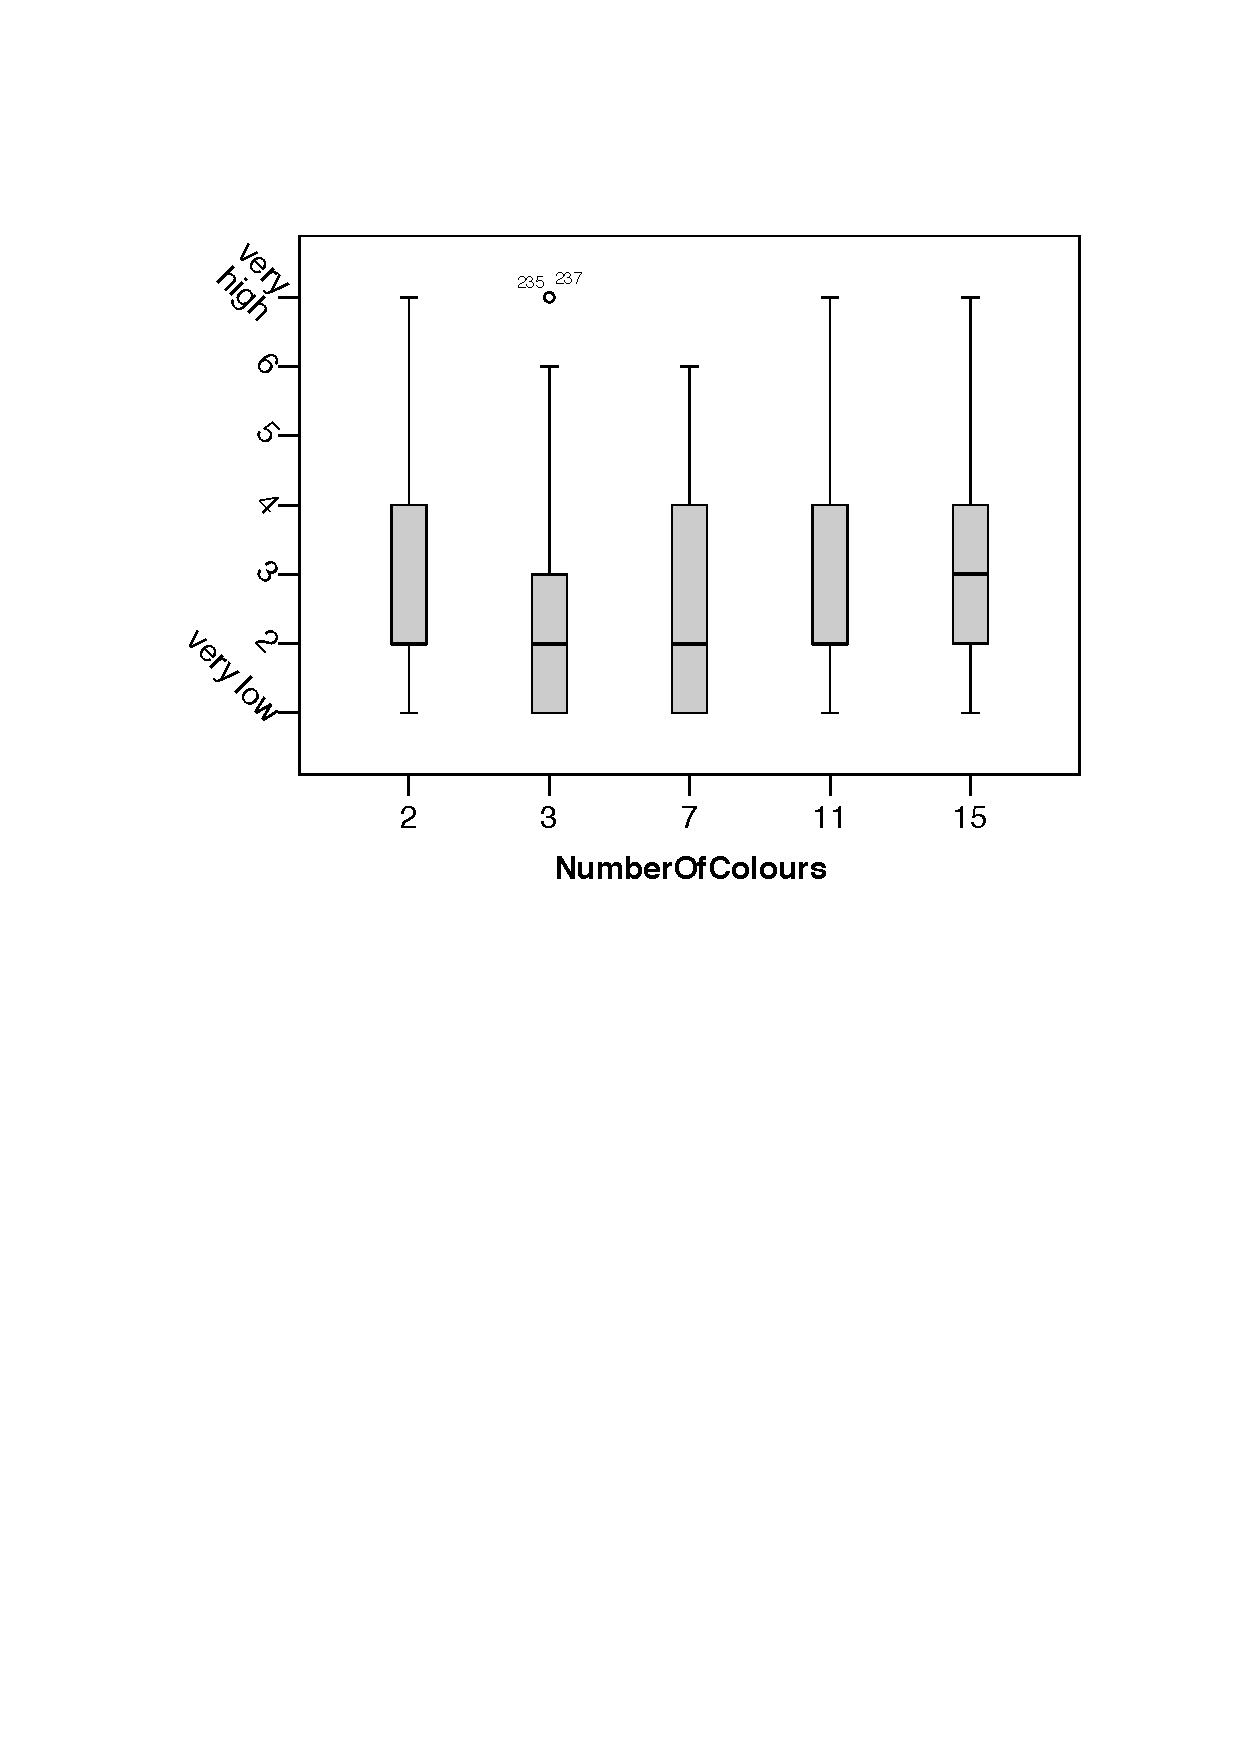
\includegraphics[height = 0.35\textwidth]{BoxplotQuestion5.pdf}
\end{subfigure}
  \caption[Question 5 - Histogram and Box plot]{Question 5 - very low (1) to very high (7)}
    \label{Question5} 
\end{center}
\end{figure}
\begin{figure}[htbp] % Question6	
\begin{center} 
\begin{subfigure} 
\centering
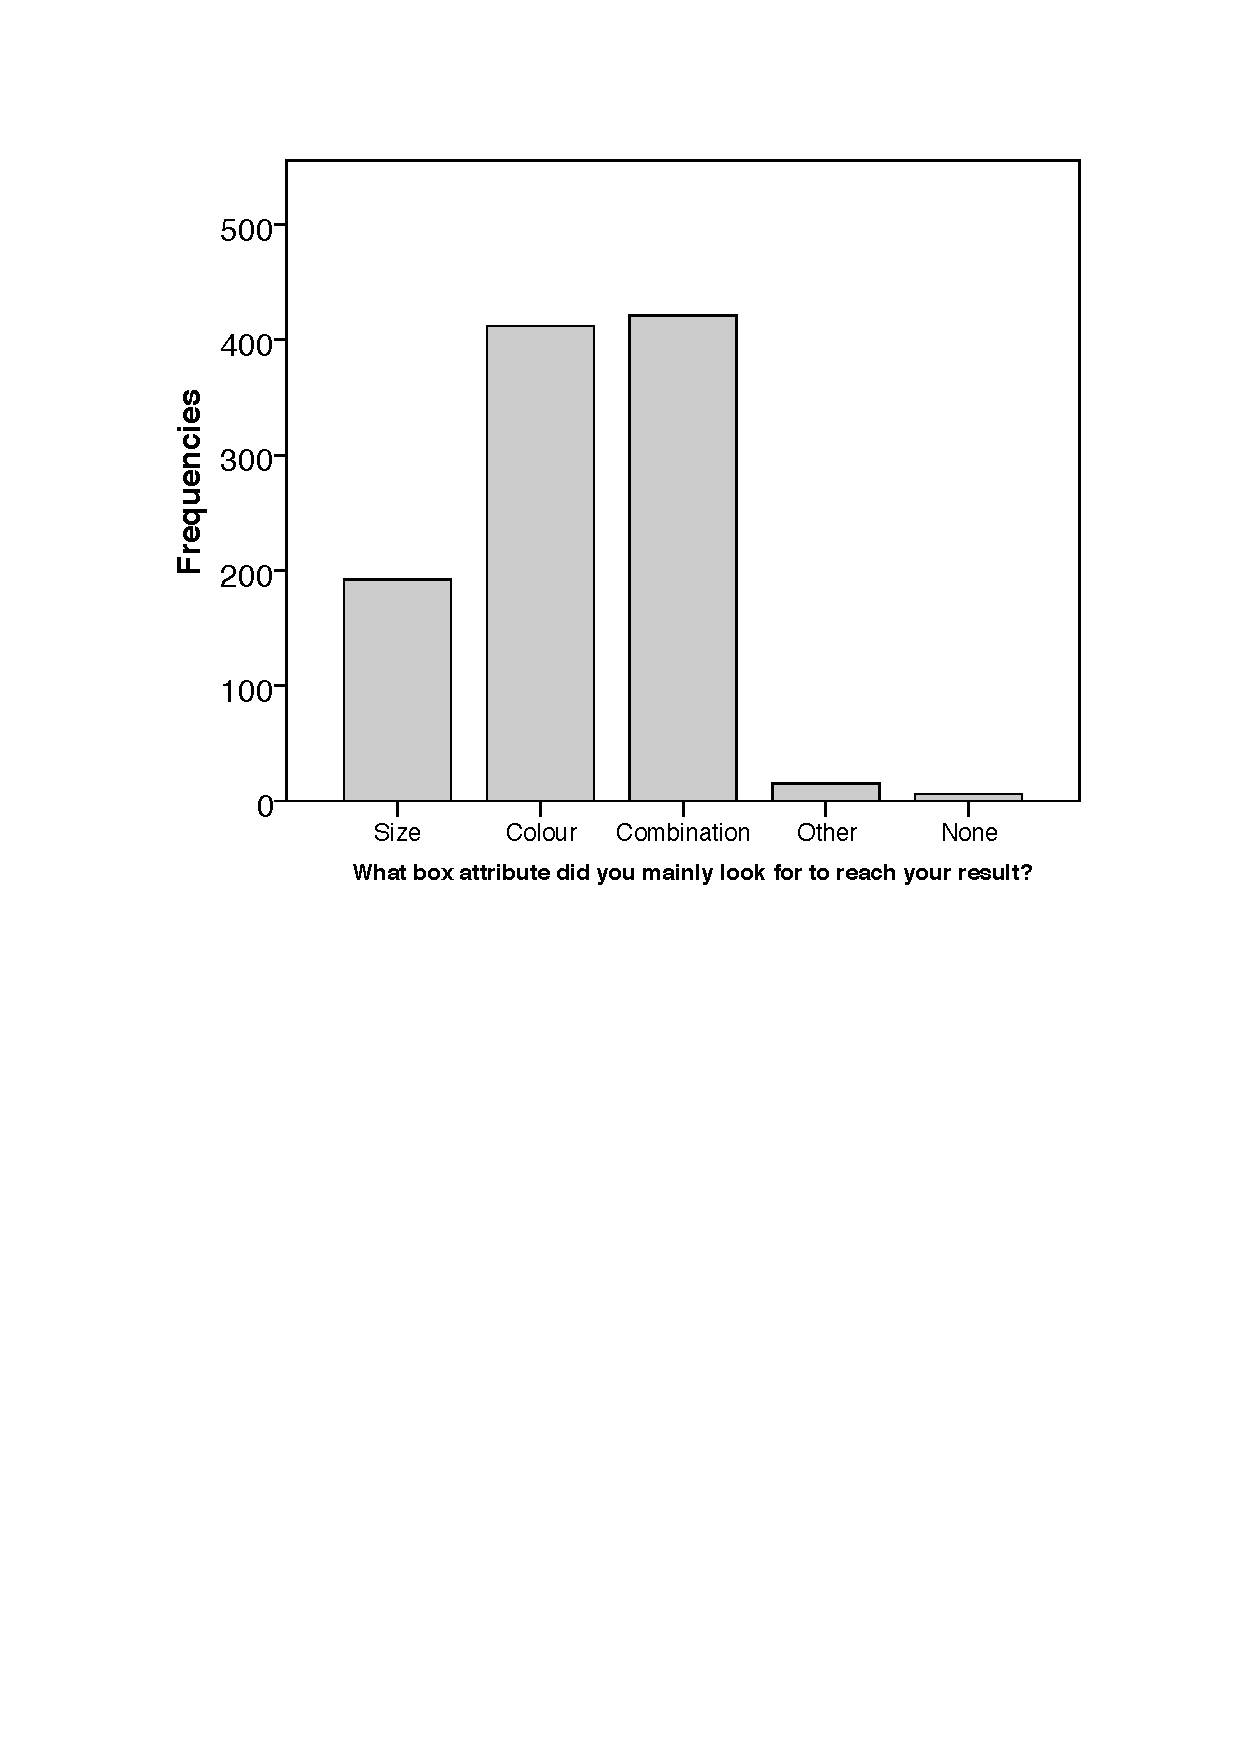
\includegraphics[height = 0.38\textwidth]{HistogramQuestion6.pdf}
\end{subfigure} 
\begin{subfigure} 
\centering
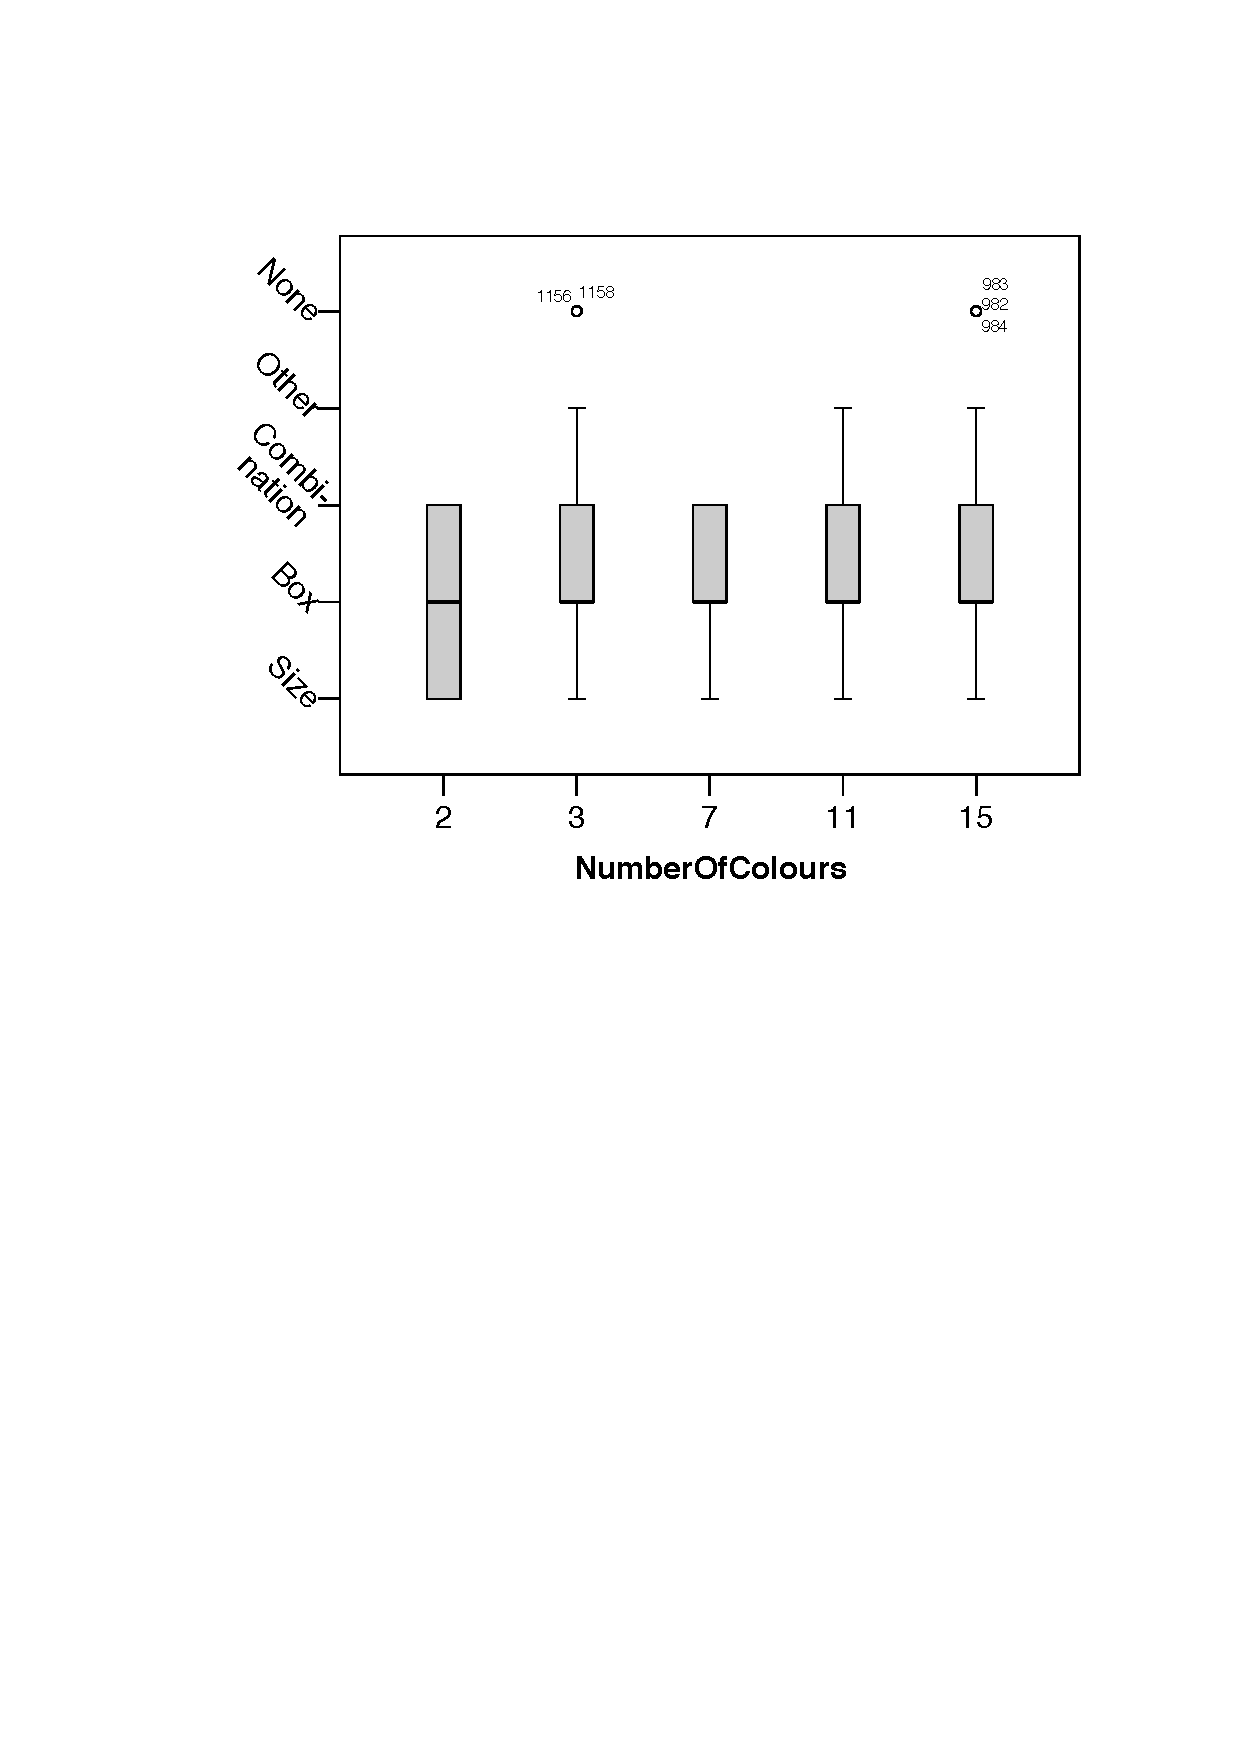
\includegraphics[height = 0.38\textwidth]{BoxplotQuestion6.pdf}
\end{subfigure}
  \caption[Question 6 - Histogram and Box plot]{Question 6 - Size (1), Colour (2), Combination (3), Other (4), None (5)}
    \label{Question6} 
\end{center}
\end{figure}
		
% Table generated by Excel2LaTeX from sheet 'Sheet1'
\begin{landscape}
\begin{table}[htbp]
  \centering
  \caption{Descriptive Statistics}
  \label{tab:DescriptiveStatistics}%
    \begin{tabular}{c|c|c|c|c|c|c|c|c|c|c|c}
    \multirow{2}[3]{*}{Variable} & \multirow{2}[3]{*}{Range} & \multirow{2}[3]{*}{Minimum} & \multirow{2}[3]{*}{Maximum} & \multicolumn{2}{c|}{Mean} & \multirow{2}[3]{*}{Std. Deviation} & \multirow{2}[3]{*}{Variance} & \multicolumn{2}{c}{Skewness} & \multicolumn{2}{c}{Kurtosis} \bigstrut[b]\\
          &       &       &       & Statistic & Std. Error &       &       & Statistic & Std. Error & \multicolumn{1}{c|}{Statistic} & \multicolumn{1}{c}{Std. Error} \bigstrut\\
    \hline
    FirstResult & 94    & 4     & 98    & 74.7  & 83\%  & 19.3  & 370.6 & -1.29 & 0.11  & 1.44 & 0.21 \bigstrut\\
    \hline
    BestResult & 94    & 4     & 98    & 79.0  & 80\%  & 18.6  & 344.7 & -1.58 & 0.11  & 2.44 & 0.21 \bigstrut\\
    \hline
    FinalResult & 94    & 4     & 98    & 78.3  & 82\%  & 19.0  & 360.0 & -1.51 & 0.11  & 2.12 & 0.21 \bigstrut\\
    \hline
    \end{tabular}%
  \label{tab:addlabel}%
\end{table}%
%\begin{table}[htbp]
%\\
%
%  \centering
%\setlength\doublerulesep{0pt}
%    \caption{Correlation Result - NumberOfColours - Round - ResultTime}
%      \label{tab:Correlation}%
%
%    \begin{tabular}{c|c|c|c|c|c|c|c|c|c}
%    \multirow{2}[0]{*}{Variable} & \multirow{2}[0]{*}{Correlation} & Number of & \multirow{2}[0]{*}{Round} & \multirow{2}[0]{*}{FirstResult} & \multirow{2}[0]{*}{BestResult} & \multirow{2}[0]{*}{FinalResult} & FirstResult & BestResult & FinalResult \\
%          &       & Colours &       &       &       &       & Time  & Time  & Time \\
%          \hline \hline
%    \multirow{2}[1]{*}{FirstResult} & Spearman's rho & -,137** & .033  & \multirow{2}[1]{*}{} & ,927** & ,924** & ,633** & ,425** & ,287** \\
%          & Pearson Correlation & -,108* & .061  &       & ,942** & ,940** & ,522** & ,399** & ,320** \bigstrut[b]\\
%    \hline
%    \multirow{2}[2]{*}{BestResult} & Spearman's rho & -,131** & .040  & ,927** & \multirow{2}[2]{*}{} & ,993** & ,564** & ,540** & ,402** \bigstrut[t]\\
%          & Pearson Correlation & -,093* & .059  & ,942** &       & ,993** & ,456** & ,509** & ,424** \bigstrut[b]\\
%    \hline
%    \multirow{2}[2]{*}{FinalResult} & Spearman's rho & -,129** & .040  & ,924** & ,993** & \multirow{2}[2]{*}{} & ,556** & ,528** & ,363** \bigstrut[t]\\
%          & Pearson Correlation & -,092* & .056  & ,940** & ,993** &       & ,458** & ,502** & ,383** \bigstrut[b]\\
%    \hline
%    \multirow{2}[2]{*}{FirstResultTime} & Spearman's rho & -.076 & -,109* & ,633** & ,564** & ,556** & \multirow{2}[2]{*}{} & ,667** & ,544** \bigstrut[t]\\
%          & Pearson Correlation & -.061 & -,106* & ,522** & ,456** & ,458** &       & ,653** & ,553** \bigstrut[b]\\
%\hline
%\cline{2-10}    \multirow{2}[2]{*}{BestResultTime} & Spearman's rho & -.021 & -.073 & ,425** & ,540** & ,528** & ,667** & \multirow{2}[2]{*}{} & ,788** \bigstrut[t]\\
%          & Pearson Correlation & -.019 & -.072 & ,399** & ,509** & ,502** & ,653** &       & ,791** \bigstrut[b]\\
%    \hline
%    \multirow{2}[2]{*}{FinalResultTime} & Spearman's rho & -.035 & -.037 & ,287** & ,402** & ,363** & ,544** & ,788** & \multirow{2}[2]{*}{} \bigstrut[t]\\
%          & Pearson Correlation & -.036 & -.038 & ,320** & ,424** & ,383** & ,553** & ,791** &  \bigstrut[b]\\
%    \hline \hline
%    \multicolumn{9}{c}{* p < 0.05, ** p < 0.01 level (2-tailed)} \bigstrut\\
%    \end{tabular}%
%\end{table}%
\end{landscape}

%\begin{landscape}
%% Table generated by Excel2LaTeX from sheet 'Sheet1 (2)'
%\begin{table}[htbp]
%  \centering
%  \caption{Correlation Question - Result - NumberOfColours}
%    \label{tab:CorrelationQuestion}%
%    \begin{tabular}{c|c|c|c|c|c|c|c|c|}
%    \multirow{2}[0]{*}{Variable} & \multirow{2}[0]{*}{Correlation} & Number of & \multirow{2}[0]{*}{FirstResult} & \multirow{2}[0]{*}{BestResult} & \multirow{2}[0]{*}{FinalResult} & FirstResult & BestResult & FinalResult \\
%          &       & Colours &       &       &       & Sqr   & Sqr   & Sqr \\
%          \hline \hline
%    \multirow{2}[1]{*}{Question 1} & Spearman's rho & \multirow{2}[1]{*}{0} & \multirow{2}[1]{*}{-- -- **/**} & \multirow{2}[1]{*}{-- -- **/**} & \multirow{2}[1]{*}{-- -- **/**} & \multirow{2}[1]{*}{-- -- **/**} & \multirow{2}[1]{*}{-- -- **/**} & \multirow{2}[1]{*}{-- -- **/**} \\
%          & Pearson Correlation &       &       &       &       &       &       &  \bigstrut[b]\\
%    \hline
%    \multirow{2}[2]{*}{Question 2} & Spearman's rho & \multirow{2}[2]{*}{0} & \multirow{2}[2]{*}{0} & \multirow{2}[2]{*}{0} & \multirow{2}[2]{*}{0} & \multirow{2}[2]{*}{0} & \multirow{2}[2]{*}{0} & \multirow{2}[2]{*}{0} \bigstrut[t]\\
%          & Pearson Correlation &       &       &       &       &       &       &  \bigstrut[b]\\
%    \hline
%    \multirow{2}[2]{*}{Question 3} & Spearman's rho & \multirow{2}[2]{*}{0} & \multirow{2}[2]{*}{+ */*} & \multirow{2}[2]{*}{+ */*} & \multirow{2}[2]{*}{+ */*} & \multirow{2}[2]{*}{+ */*} & \multirow{2}[2]{*}{+ */*} & \multirow{2}[2]{*}{+ */*} \bigstrut[t]\\
%          & Pearson Correlation &       &       &       &       &       &       &  \bigstrut[b]\\
%    \hline
%    \multirow{2}[2]{*}{Question 4} & Spearman's rho & \multirow{2}[2]{*}{0} & \multirow{2}[2]{*}{-- -- **/**} & \multirow{2}[2]{*}{-- -- **/**} & \multirow{2}[2]{*}{-- -- **/**} & \multirow{2}[2]{*}{-- -- **/**} & \multirow{2}[2]{*}{-- -- **/**} & \multirow{2}[2]{*}{-- -- **/**} \bigstrut[t]\\
%          & Pearson Correlation &       &       &       &       &       &       &  \bigstrut[b]\\
%    \hline
%    \multirow{2}[2]{*}{Question 5} & Spearman's rho & \multirow{2}[2]{*}{+ **/**} & \multirow{2}[2]{*}{-- */*} & \multirow{2}[2]{*}{-- */*} & \multirow{2}[2]{*}{-- */*} & \multirow{2}[2]{*}{-- */*} & \multirow{2}[2]{*}{-- */*} & \multirow{2}[2]{*}{-- */*} \bigstrut[t]\\
%          & Pearson Correlation &       &       &       &       &       &       &  \bigstrut[b]\\
%    \hline
%    \multicolumn{9}{c}{** p<0.01, * p<0.05, ++ <0.3, + <0.2, [0.1,-0.1] 0, -- > --0.2, -- -- > -- 0.3} \bigstrut[t]\\
%    \end{tabular}%
%\end{table}%
%\end{landscape}